\chapter{Event Selection:\\Baseline and Search regions}
\label{Chap:eventSel}
%\minitoc
\section{SUSY signature}
\label{signalDef}
As mentioned in Sec.~\ref{sec:simplifiedModels}, a search for SUSY is performed in the context of the simplified model T5qqqqWW (see Fig.~\ref{fig:T5qqqqWW})\footnote{Throughout this thesis, the T5qqqqWW model is referred to the signal model.}. In this model, each gluino decays to two light quarks~($c$,$s$,$u$,$d$) and an intermediate chargino, with the latter decaying to a $W$ boson and a neutralino.\\
\begin{figure*}[!hb]
  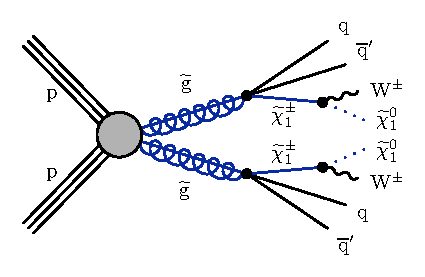
\includegraphics[width=0.5\textwidth]{Plots/feyndiagrams/T5qqqqWW.pdf}
\centering
  \caption{\label{fig:T5qqqqWW} Diagram of the the simplified model T5qqqqWW. 
  }
\end{figure*}
The event selection is designed to have the largest possible signal efficiency hence it is related to expected final state of the SUSY signal signature.\\
In the event selection, one of the W bosons is chosen to be decaying leptonically. The choice of single lepton final states provides a cleaner event topology than the full hadronic final states while keeping the signal efficiency sufficiently high. The visible final state includes then at least six jets and one lepton~(either electron or muon). In order not to loose events where two jets with high energy are produced aligned and reconstructed as one jet, or jet out of acceptance, the jet multiplicity is required to be at least five. Moreover, as a distinct feature of this model, it is required that none of the jets are tagged as originating from b quark. Furthermore, in such events, a high $\MET$ is expected due to the presence of the neutralino and the neutrino which leave no trace in the detector.\\ 
%These selections can be further enhanced by  the characteristics of individual objects such as; the transverse momentum of lepton $p_{T,\ell}$ or jets $p_{T, jets}$. or using object characteristics 
Merely selecting events with one lepton, five jets, and high $\MET$ is not enough to reveal the existence of SUSY-like events which are rare among the many SM like events with similar final states. The $\wJets$ and $\ttJets$ events are the leading SM background processes which can mimic the T5qqqqWW signature. Therefore, some advanced kinematic variables need to be defined to eliminate these SM background processes.
%Table \ref{tab:KinVar} shows the list of variables which are employed. This list does not include the variables that are used in the identification of particle flow objects (see Sec. \ref{sec:PF}). The physics variables are categorized according to their mathematical complexity.\\
%\renewcommand{\arraystretch}{1.5}
%\begin{table}[ht]
%\begin{center}
%\begin{tabular}{|c|c|}\hline
%Simple variables        & Advanced variables \\
%\hline
%\hline
%$L_T$ , $H_T$ & $\Delta\Phi(W,\ell)$ \\
%$p_{T,\ell}$ , $\eta_{\ell}$& $\MTt(\vec{p}_{\text T}^{\,\ell},\vec{p}_{\text T}^{\,t},\ptvecmiss)$  \\
%$p_{T,jets\,(1,2)}$ & \\
%$n_{jets}$ & \\
%$n_{b-tag}$ & \\
%\hline
%\end{tabular}
%\end{center}
%\caption{List of kinematic variables}\label{tab:KinVar}
%\end{table}
%\renewcommand{\arraystretch}{1}
\subsection{Key variables}
\label{keyVars}
The list of variables consists of fundamental properties of the reconstructed particles, such as the transverse momentum $\pt$ of these objects, and functions of them. The reconstruction and identification of these particles are introduced in Ch.\ref{Ch:ObjectsDef}.\\
%\boldmath
\begin{itemize}
\item {\boldmath $\njet$} is the number of all jets  above a $p_T$ threshold in an event.
\item {\boldmath $\nbtag$} is the number of all jets tagged as coming from a b quark above a $\pt$ threshold, as with other jets, in the event.
\item {\boldmath $\HT$}, $\sum \pt({\rm jets})$,  is the scalar sum of the transverse momenta of all jets above a $\pt$ threshold in the event. For signal events, the major contribution to this sum is coming from transverse energy of the jets originated from the gluino decay, and it is related to the mass gap between the gluino and the chargino. This variable reflects the "hadronic mass scale" of the event.
\item {\boldmath $\LT$} is the scalar sum of the charged lepton $\pt$ and the missing transverse momentum $\MET$.
Given no additional source of $\MET$, except the SM neutrino, the variable $\LT$ can be also written as: $\sqrt{p_{\rm T(W)}^2+M_{\rm T(W)}^2}$. The derivation of this relation starts by expanding the squared transverse momentum and the transverse mass of the W boson:
\begin{eqnarray}
{p_{\rm T(W)}^2} = {(p_{\rm T(\ell)}\cdot \cos\phi_{\ell} + \MET \cdot \cos \phi_{\MET})^2+(p_{\rm T(\ell)}\cdot \sin\phi_{\ell} + \MET \cdot \sin \phi_{\MET})^2},\nonumber \\
{M_{\rm T(W)}^2} = {2\cdot p_{\rm T(\ell)}\cdot\MET\cdot(1-(\cos\phi_{\MET} \cdot \cos\phi_{\ell} +\sin\phi_{\MET}  \cdot \sin\phi_{\ell} ))},\nonumber \\
{p_{\rm T(W)}^2+M_{\rm T(W)}^2}  = {p_{\rm T(\ell)}^2+\MET^2+2\cdot p_{\rm T(\ell)}\cdot\MET\cdot(\cos\phi_{\MET} \cdot \cos\phi_{\ell} +\sin\phi_{\MET}  \cdot \sin\phi_{\ell} ) \nonumber\\
-2\cdot p_{\rm T(\ell)}\cdot\MET\cdot(\cos\phi_{\MET} \cdot \cos\phi_{\ell} +\sin\phi_{\MET}  \cdot \sin\phi_{\ell} )+2\cdot p_{\rm T(\ell)}\cdot\MET},\nonumber \\
{(p_{\rm T(\ell)}+\MET)^2} = {\LT^2}.
  \label{eq:LTderive}
\end{eqnarray}
For events with a single boosted W boson ($p_{\rm T(W)}\gg M_{\rm T(W)}$), $\LT \sim p_{\rm T(W)}$. This variable is also known as "leptonic mass scale" of the event.
\item {\boldmath $\DFWL$} is the azimuthal angle between the W boson candidate, formed from the $\MET$ and lepton $\ptvec$, and the charged lepton. In $\wJets$ and $\ttJets$ background events, the lepton comes from a leptonic decay of the W boson, ${\rm W\rightarrow\ell\nu}$, which strongly constraints allowed values for $\DFWL$. It is small when the daughter particle is aligned with its mother as in the case of single leptonic $\wJets$ and $\ttJets$ events.
%In SM events with high missing energy indicates that the $W$ bosons yielding the lepton and the neutrino are boosted, hence resulting in a narrow distribution in $\Delta\Phi(W,\ell)$. 
On the other hand, in SUSY decays, the missing transverse energy comes from two neutralinos and the neutrino, which randomizes $\DFWL$, thus resulting in an almost flat distribution, making $\DFWL$ a highly discriminating observable.
%This angle show similar behaviour to the transverse mass of the lepton and $\MET$, with a better resolution.
The high values of $\DFWL$ are used as a signal region\footnote{where signal to background event counts are sufficiently large.} while the low values of $\DFWL$ are the control region\footnote{where signal event counts are negligible with respect to background event counts.}.
\item {\boldmath $\MTt$}~\cite{MT2} is defined as:
\begin{eqnarray}
  \MTt(\vec{p}_{\text T}^{\,\ell},\vec{p}_{\text T}^{\,t},\ptvecmiss) =
  \min\limits_{\vec{p}_{\text T}^{(1)}+\vec{p}_{\text T}^{(2)} = \ptvecmiss} \left\{
  \max \left[ \MT(\vec{p}_{\text T}^{\,\ell}, \vec{p}_{\text T}^{(1)}), 
              \MT(\vec{p}_{\text T}^{\,t},\vec{p}_{\text T}^{(2)})\right] \right\},
  \label{eq:MT2}
\end{eqnarray}
where $\MT$ is the transverse mass and the indices $t$,$\ell$ represent an isolated track and the selected lepton respectively. This variable is used only in the baseline selection to reduce contributions with a second, unidentified electron or muon, or the hadronic decay of a tau lepton. It reduces the dileptonic $\ttJets$ contribution which is more important in the signal region~(high  $\DFWL$). 
\end{itemize}
\subsection{Signal samples}
\label{signalSamples}
The simplified model T5qqqqWW is discussed in Sec.~\ref{sec:simplifiedModels}. This model in principle includes three free mass parameters\footnote{there are many more parameters that are ignored}: the masses of the gluino $m_{\tilde{g}}$, the intermediate chargino $m_{\chipmone}$ and the neutralino $m_{\ninoone}$. To reduce the three dimensional mass space the chargino mass is fixed to the arithmetic mean of gluino and neutralino mass. For each mass point, a separate MC sample is produced. The complete mass plane is shown in  Fig.\ref{fig:massplane} where the z-axis represents the total number of events generated. The $\MADGRAPH$5 event generator is used for signal events modelling. The scan of parameter space includes 657 mass points which are simulated using FastSim (Sec.~\ref{sec:forFastsim}) in order to reduce CPU consumption. The samples are normalized according to the gluino production cross section~\cite{gluxsec2}.
Two mass points corresponding to different gluino and neutralino masses are used as benchmarks to study the kinematic properties of the signal.
\begin{itemize}
\item \textbf{T5qqqqWW(1.9,0.1)} represents a point in the high mass gap region with $m_{\tilde{g}}=$~1900~GeV and $m_{\ninoone}=$~100~GeV. These signal events have high $\HT$ and $\LT$.
\item \textbf{T5qqqqWW(1.5,1.0)} represents a point close to the compressed region with $m_{\tilde{g}}=$~1500~GeV and $m_{\ninoone}=$~1000~GeV. The compressed region is where the $m_{\tilde{g}}-m_{\ninoone}\leq2\,m_{\rm W}$. These signal events have lower {\HT} and {\LT} with respect to high mass gap ones.
\end{itemize}
In Fig.~\ref{fig:signalKin}, $\HT$~(left), $\LT$~(middle), $\njet$~(right) distributions for three different signal mass points are shown. When the mass gap between gluino and neutralino is low, it results in softer hadronic and leptonic activity and vice~versa.\\
\begin{figure*}[!h]
\centering
  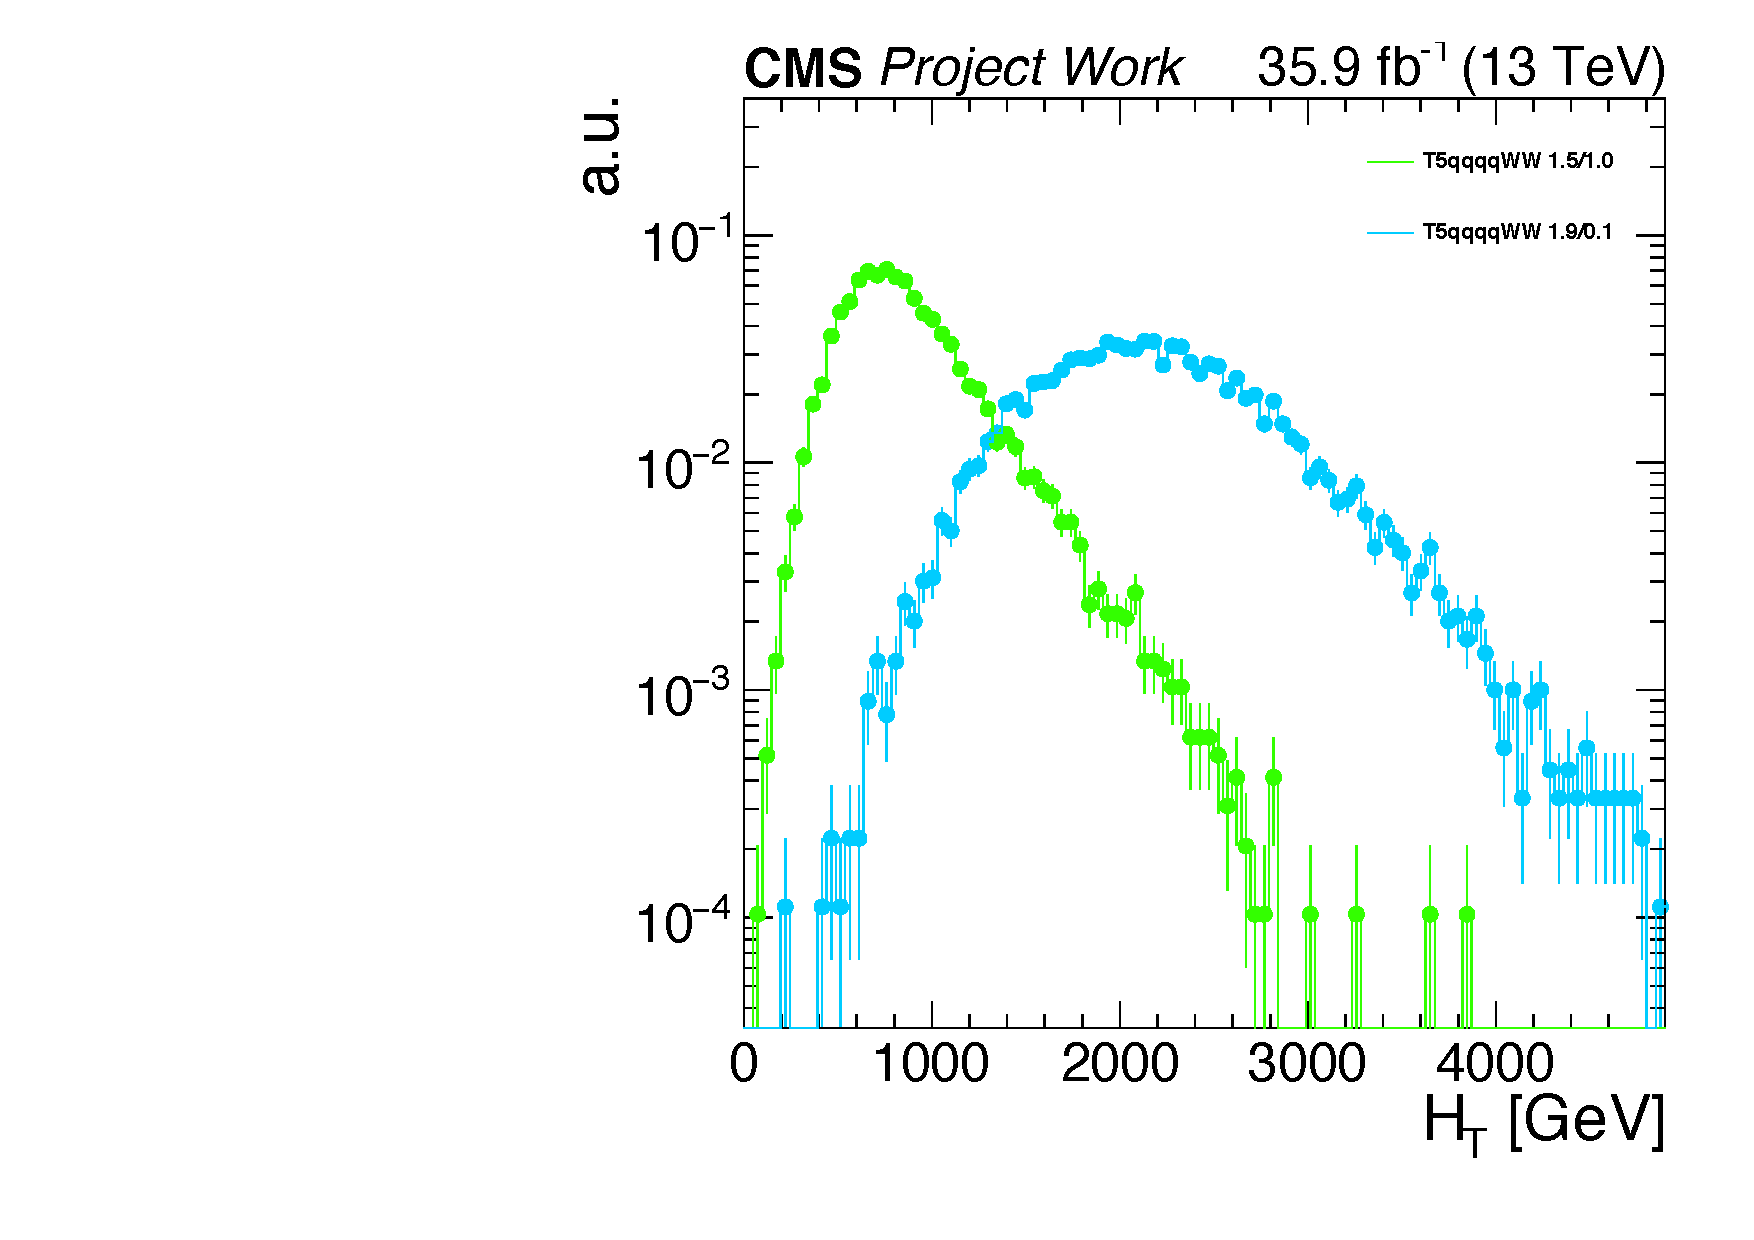
\includegraphics[width=0.3\textwidth]{PhD_Thesis_v4/Plots/signals/HT2.pdf}
  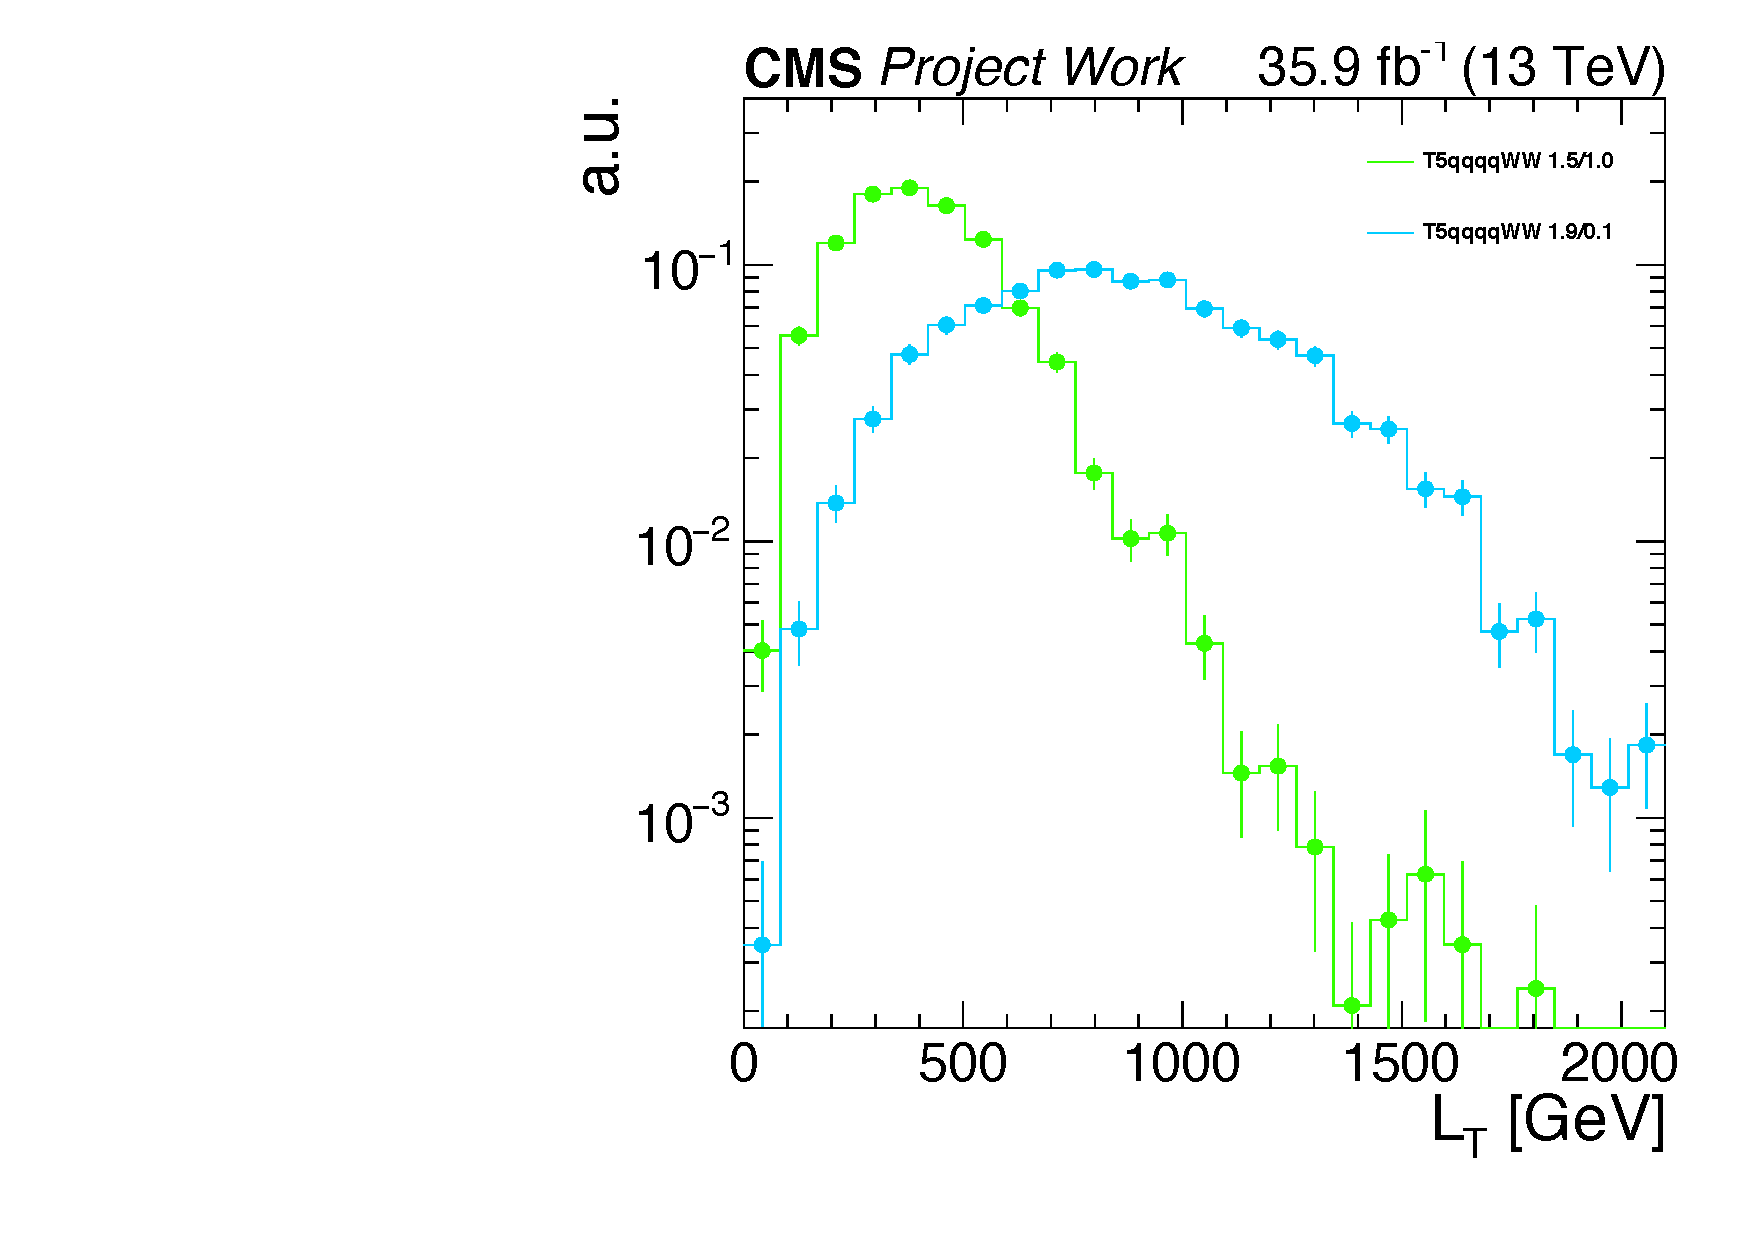
\includegraphics[width=0.3\textwidth]{PhD_Thesis_v4/Plots/signals/LT2.pdf}
  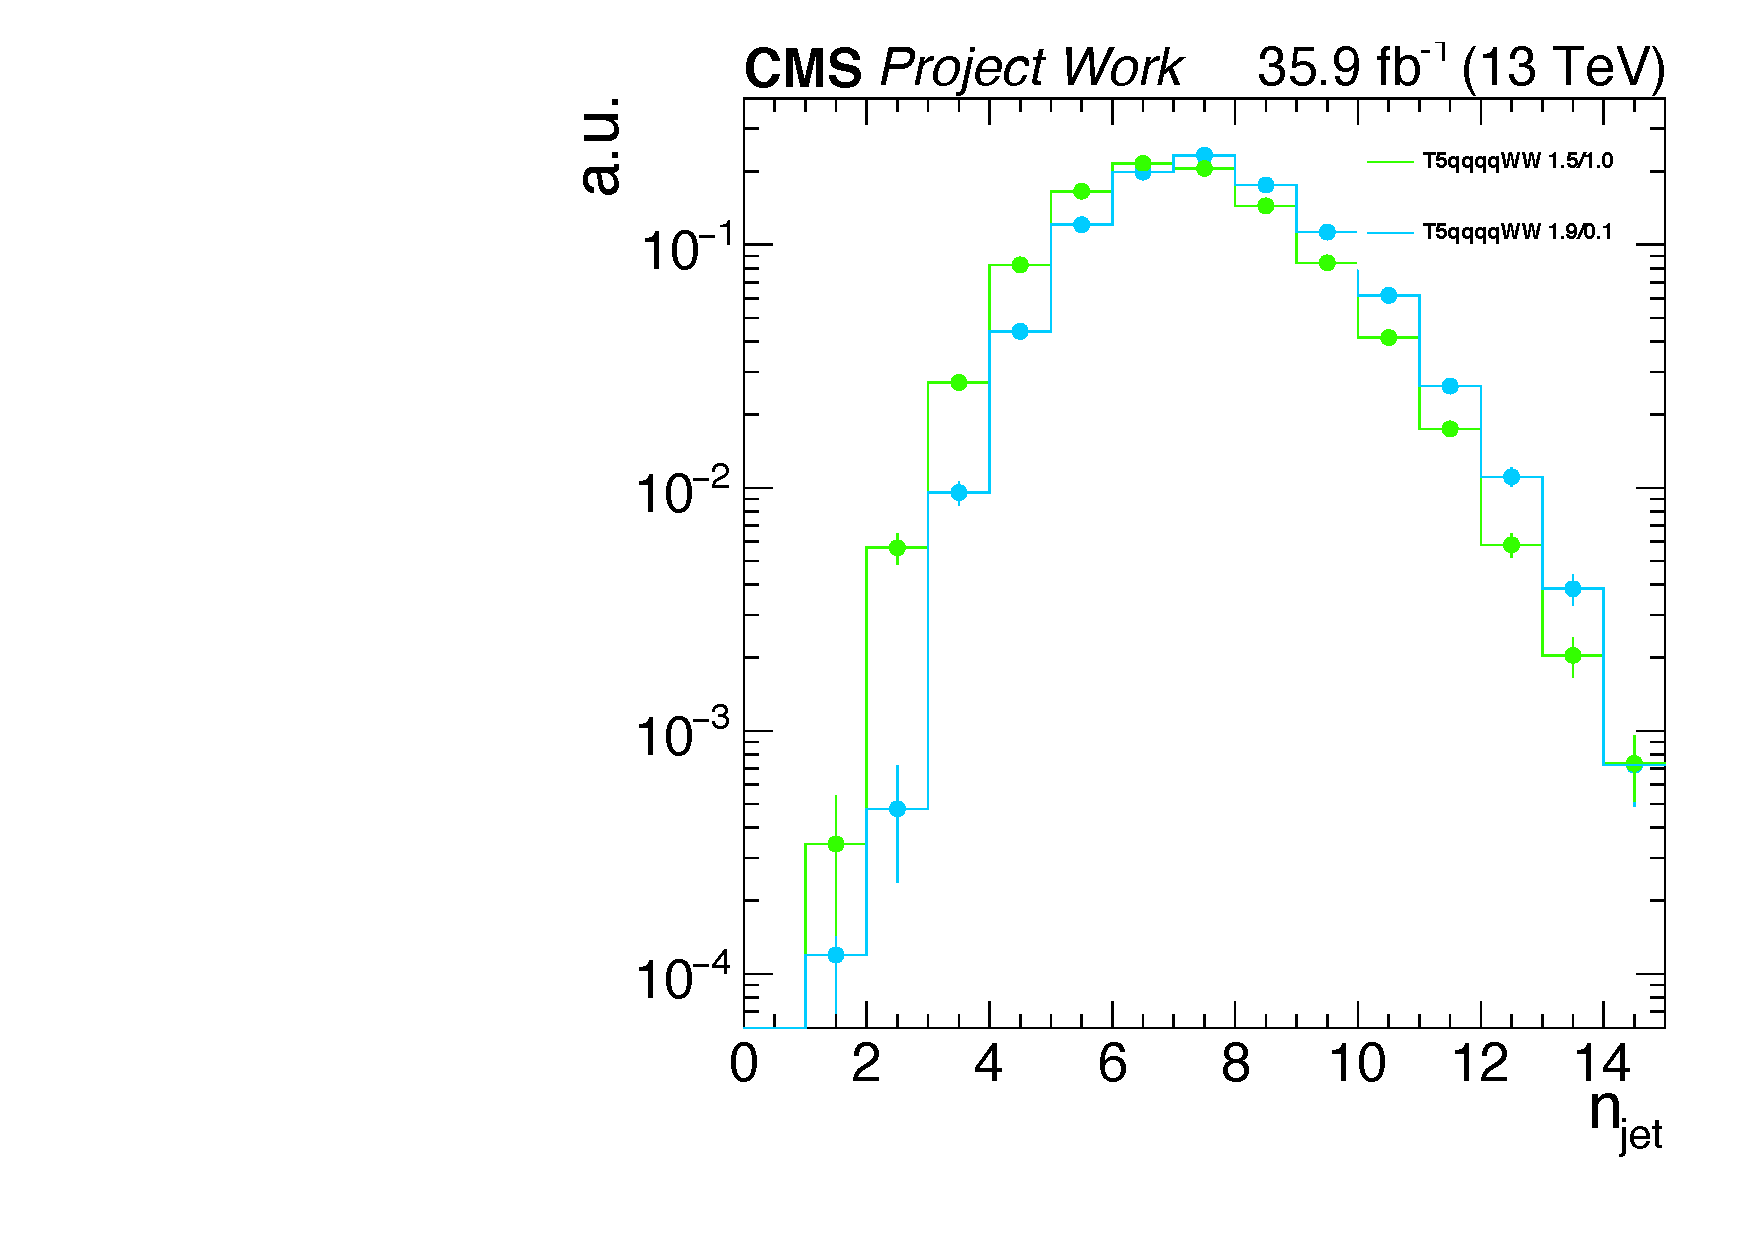
\includegraphics[width=0.3\textwidth]{PhD_Thesis_v4/Plots/signals/nJet2.pdf}
  \caption[$\HT$~(left), $\LT$~(middle), $\njet$~(right) distributions for three different signal mass point]{\label{fig:signalKin}  $\HT$~(left), $\LT$~(middle), $\njet$~(right) distributions for three different signal mass point. Distributions are normalized to one. The green line represents the low mass gap signal point ($m_{\tilde{g}}=$~1.4~TeV and $m_{\ninoone}=$~1.0~TeV), the light blue line shows the high mass gap ($m_{\tilde{g}}=$1.9~TeV and $m_{\ninoone}=$~0.1~TeV) benchmark point.
  }
\end{figure*}
\begin{figure*}[!h]
  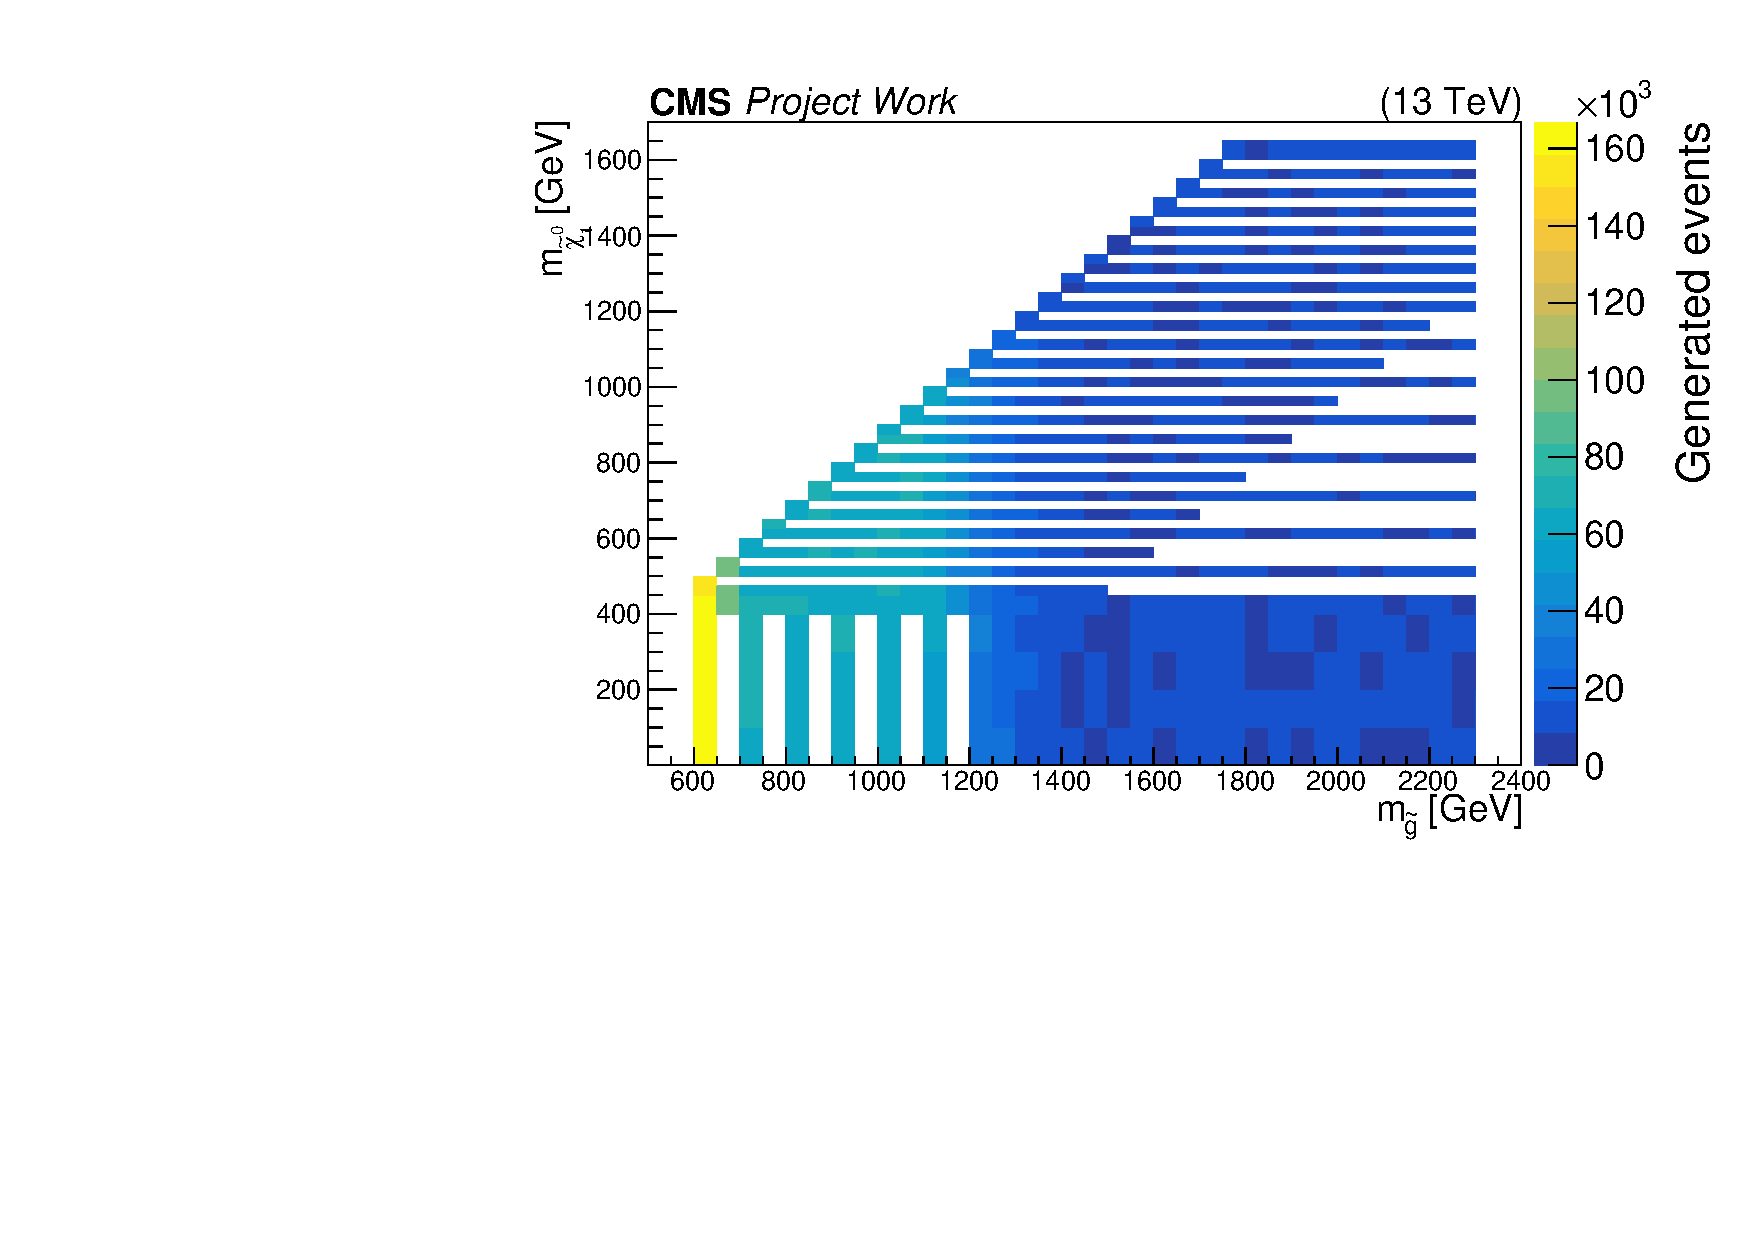
\includegraphics[width=0.7\textwidth]{Plots/signals/signal_scan.pdf}
\centering
  \caption{\label{fig:massplane} Simulated signal mass points for the simplified T5qqqqWW model.
  }
\end{figure*}
%\section{Samples}
\section{Background processes}
\label{sec:bkg_proc}
As mentioned earlier in this section, the most important background processes are $\wJets$ and $\ttJets$ events. $\wJets$ events becomes the main background, when zero b-tagged jets are required in the event selection. All of the background processes considered in this analysis are listed below.
%\begin{aligned}
\begin{itemize}
\item {\boldmath $\ttJets$} is generated with $\MADGRAPH$5\_\textsc{aMC@}NLOv2.2.2. To enhance the statistics, the combination of {\HT} binned samples, dedicated semi- and di-leptonic samples is used.
\item {\bf \wJets} is generated with $\MADGRAPH$5\_\textsc{aMC@}NLOv2.2.2. $\HT$ binned samples, where W boson decaying leptonically, are used.
\item \textbf{QCD multijet} events are produced with $\MADGRAPH$5\_\textsc{aMC@}NLOv2.2.2 in bins of $\HT$.
\item {\boldmath $\singleTop$} samples are produced with POWHEGv2.0 except for the single top quark decaying leptonically with $s$-channel is produced with NLO $\MADGRAPH$5\_\textsc{aMC@}NLOv2.2.2.
\item \textbf{\DY} events are produced with $\MADGRAPH$5\_\textsc{aMC@}NLOv2.2.2 and $m_{\ell\ell}>50 GeV$ sample is used in {\HT} bins.
\item \textbf{Di-boson} samples are produced with \textsc{aMC@}NLO except for WW samples that are produced with POWHEG.
\item {\boldmath \TTVH} samples are produced with \textsc{aMC@}NLO.
\end{itemize}
A list of all background MC samples with cross sections can be found in Appendix~\ref{sec:Appsamples}.
%\end{aligned}
%\newpage
\subsection{Scale factors}
\label{sec:SF}
Studies of data/MC ratios reveal that event-by-event scale factors are needed to remove or mitigate shortcomings of the simulation.\\
\textbf{Lepton identification and reconstruction efficiency}\\
MC samples have to be corrected according to the reconstruction and identification efficiencies of leptons.
In this work, scale factors are applied as a function of $p_{T}$ and $\eta$ of the selected lepton~\cite{leptonSF}.\\
\textbf{Efficiency and event weights of b tagging}\\
The b tagging efficiency SFs~\cite{leptonSF} are measured, ($SF=\epsilon_{\rm DATA}/\epsilon_{\rm MC}$), for b and light flavor jets as a function of jet $ \pt $ and $ \eta $. To predict the correct event yield in data, SFs are applied to the selected MC events. For the weighting of simulated events, a probabilistic approach is used. 
The probability of a jet to be b-tagged, which is denoted by $p_i$, and is measured, as a function of jet $\pt,\,\eta$ and flavor of the original parton in simulation. The index $i$ labels the jets in the event. The $p_i$ is equal to b tagging efficiency, $\epsilon_i$(Eq.~\ref{Eq.btagEff}), when the jet comes from a generated b quark.
\begin{eqnarray}
\label{Eq.btagEff}
  {\epsilon_f(\pt,\,\eta)=\frac{\rm N_f^{b-tagged}(\pt,\,\eta)}{\rm N_f^{Total}(\pt,\,\eta)}},
\end{eqnarray}
where ${\rm N_f^{b-tagged}}$ and ${\rm N_f^{Total}}$ are the number of b-tagged and all jets, respectively, for flavor $f$ in $(\pt,\,\eta)$.
The scale factors from simulation to data, $SF_i$, are applied on the b-tagging probability, $P_i=SF_i \cdot p_i$. The probability of an event to be reconstructed with exactly $n$ b-tagged jets, becomes:
%{w({\rm 0\,b-tagged\,jets})} = {\prod_{i} (1-P_i)},\\
\begin{eqnarray}
  {w({\rm n\,b-tagged\,jets})} = {\overbrace{{\cdots\sum_i\sum_j}}^\text{n}\Big[\overbrace{{\cdots P_iP_j}}^\text{n}\prod_{k} (1-P_k)\Big]}, {\rm \,with\,} {\,j>i} {\rm \,and\,} {k\neq i,j}.
\end{eqnarray}
This method allows reusing the events, because each event will contribute to any b-tag multiplicity, irrespective of the parton multiplicities. The advantage of this method is that it allows to use the full statistical power of the MC events.\\
\textbf{ISR reweighting:}\\
Since the 8 TeV Run of LHC, it is known that the $\pt$ spectrum and the number of additional jets of $\ttbar$ events are not well modeled. Therefore, an event-by-event correction is obtained using the jets from initial state radiation~(ISR).
 Each event is corrected according to number of ISR jets. The weights can be seen in Tab.~\ref{tab:nISRweights} where the factor D is selected in order to preserve the normalization of the inclusive sample.
 \renewcommand{\arraystretch}{1.5}
\begin{table}[htbp]
\begin{center}
\caption{Weights based on the number of ISR jets as given in Ref.~\cite{nISRweightTTbar}}
\begin{tabular}{|r|l|}
\hline
\multicolumn{1}{|l|}{nISR jet} & Normalisation weight $D_{\ttbar} = 1.071$ \\ \hline
0 &  \\ \hline
1 & $D \times (0.920 \pm 0.005 \pm 0.040)$ \\ \hline
2 & $D \times (0.821 \pm 0.006 \pm 0.090)$ \\ \hline
3 & $D \times (0.715 \pm 0.009 \pm 0.143)$ \\ \hline
4 & $D \times (0.662 \pm 0.016 \pm 0.169)$ \\ \hline
5 & $D \times (0.561 \pm 0.027 \pm 0.219)$ \\ \hline
$\geq$ 6& $D \times (0.511 \pm 0.041 \pm 0.244)$ \\ \hline
\end{tabular}
\label{tab:nISRweights}
\end{center}
\end{table}
\\
\renewcommand{\arraystretch}{1}
\textbf{Pileup:}\\
As discussed earlier in Sec.~\ref{sec:PV}, the number of pileup interactions in simulated samples is sampled from a prior distribution, approximately reflecting 2016 data taking conditions. Thus, the MC pileup distribution may vary from the actual pileup distribution in Data. The simulated distribution is rescaled with the Data/MC ratio in Fig.~\ref{fig:pileUpmine}, in order to achieve agreement in the true number of interactions.
\begin{figure*}[!h]
  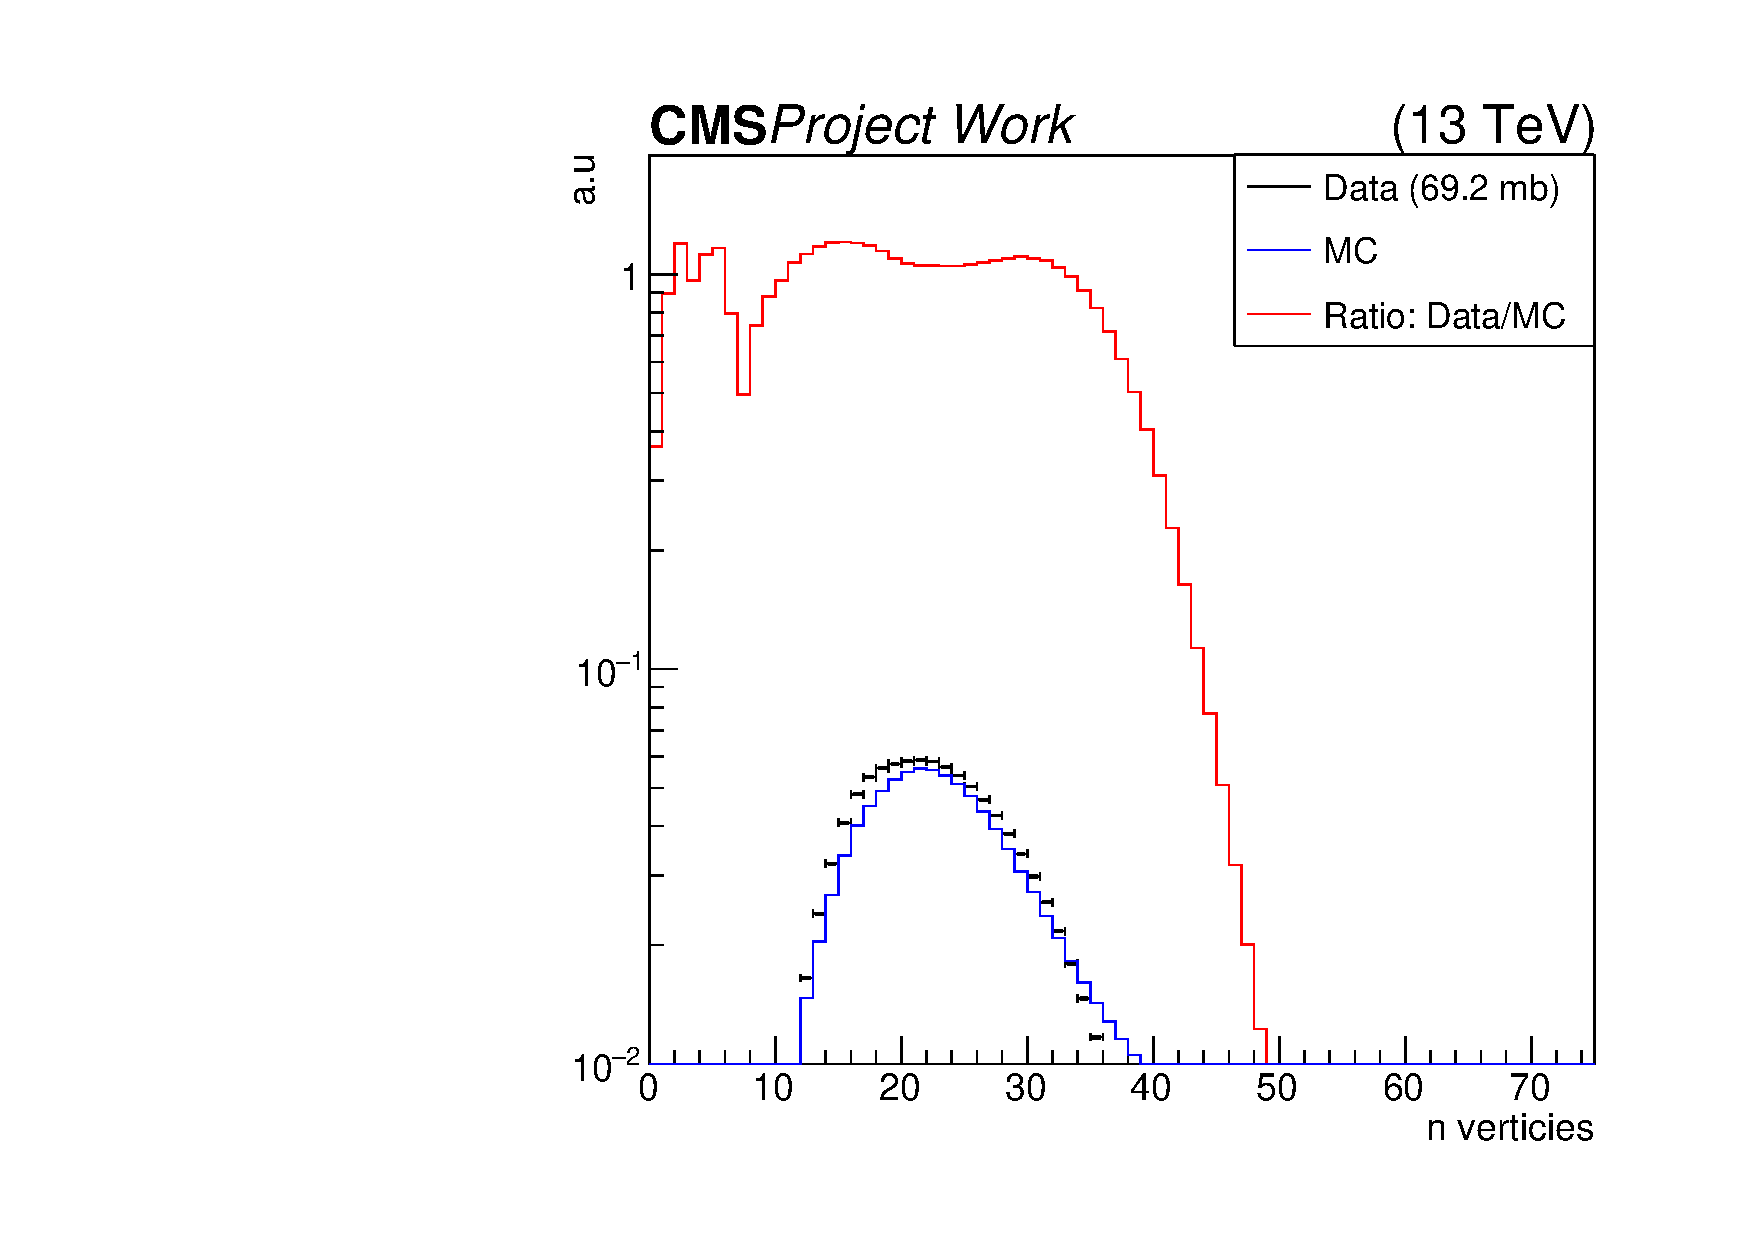
\includegraphics[width=0.5\textwidth]{PhD_Thesis_v4/Plots/analysis/pileUp/pileup.pdf}
\centering
  \caption[The normalized distributions of mean number of interactions per bunch crossing]{\label{fig:pileUpmine} The normalized distributions of mean number of interactions per bunch crossing during the analyzed data Run2016 (black) and in the MC samples (blue). The red distribution represents the Data to MC ratio. For the data distribution the latest luminosity calibrations~\cite{pileupCMS} and an inelastic pp cross-section of 69.2~mb are used. 
  }
\end{figure*}
\newpage
\section{Baseline selection}
\label{sec:BL}
%Earlier in this Sec.~\ref{signalDef}, the targeted SUSY signature is introduced. Moreover, for removing the SM background as much as possible while keeping a high signal efficiency, a suitable primary event selection was discussed.
Object selections have been discussed in Sec.~\ref{Ch:ObjectsDef} and are now used to define the event selection.\\
\textbf{Selections on leptons}\\
Exactly one lepton~(electron or muon) is selected. The selected lepton is required to have a minimum $\pt$ of 25 GeV while at the same time it satisfies the tight lepton criteria introduced in Sec.\ref{sec:PFleptons}. Additionally, events are vetoed if there is an extra lepton with $\pt>$~10 that satisfies the loose lepton selection criteria.\\
\textbf{Selections on jets}\\
Jets are required to have $\pt > 30$~GeV and $| \eta | < 2.4 $. Furthermore, in order to avoid double counting of objects, jets that are close ($\Delta R <0.4$) to either a veto or selected lepton are removed.
As discussed earlier in this chapter, the T5qqqqWW model is expected to have at least five jets. The mass difference of the gluino and the intermediate chargino affects the typical $\pt$ of the jets. Therefore, it is moreover required that two highest $\pt$ jets satisfy $\pt >80$ GeV. Additionally, in the baseline selection, the number of jets tagged as coming from b quarks is required to be zero in order to suppress the events containing top quarks.
\\
\textbf{Energy scales thresholds}\\
The signal model favors events with high $\HT$ and $\LT$ as can be seen in Fig.~\ref{fig:signalKin}. The $\HT$ is chosen to be at least 500~GeV while the $\LT$ threshold is 250~GeV.
\\
\textbf{Isolated track veto}\\
To suppress $\ttbar$ events in which both W bosons decay leptonically and one lepton does not satisfy the selection criteria for veto leptons, events that contain at least one isolated high-$\pt$ charged track are rejected. These tracks originate from $\tau \rightarrow \nu_{\tau}+{\rm hadron}$ decays~(hadronic tracks) or electron or muon tracks~(leptonic tracks) of poor quality. For this veto, the $\MTt$ variable, which is introduced in Sec.~\ref{keyVars}, is used with an isolated track $t$, a lepton $\ell$ and the missing transverse momentum $\ptvecmiss$. In the calculation of $\MTt$, it is assumed that the missing energy comes from the two neutrinos from the dileptonic $\ttbar$ decay. The minimization runs over all possible splitting of $\ptvecmiss$.
Figure~\ref{fig:track_mt2} shows the $\MTt$ distribution separate for hadronic and leptonic tracks after the baseline selection with $\HT > 500$~GeV, $\LT > 250$~GeV,  $\njet \geq 5$ and without b tag requirement. The distribution of {\MTt\,} is slightly different for the two cases and a lower {\MTt\,} cut of $60$ GeV and $80$ GeV is applied for hadronic and leptonic tracks respectively. The rightmost plot in  the Fig.~\ref{fig:track_mt2}
shows the \MTt\, distribution for all events i.e. including events that do not have any isolated track at all. In this case events without any isolated track are added to the overflow bin. It can also be seen that only about 20\% of the signal events have an opposite charged isolated track at all compared to 40\% of the dileptonic $\ttbar$ events.
 \begin{figure*}[!h]
    \begin{center}
  \subfigure[\MTt\, with leptonic tracks]{ 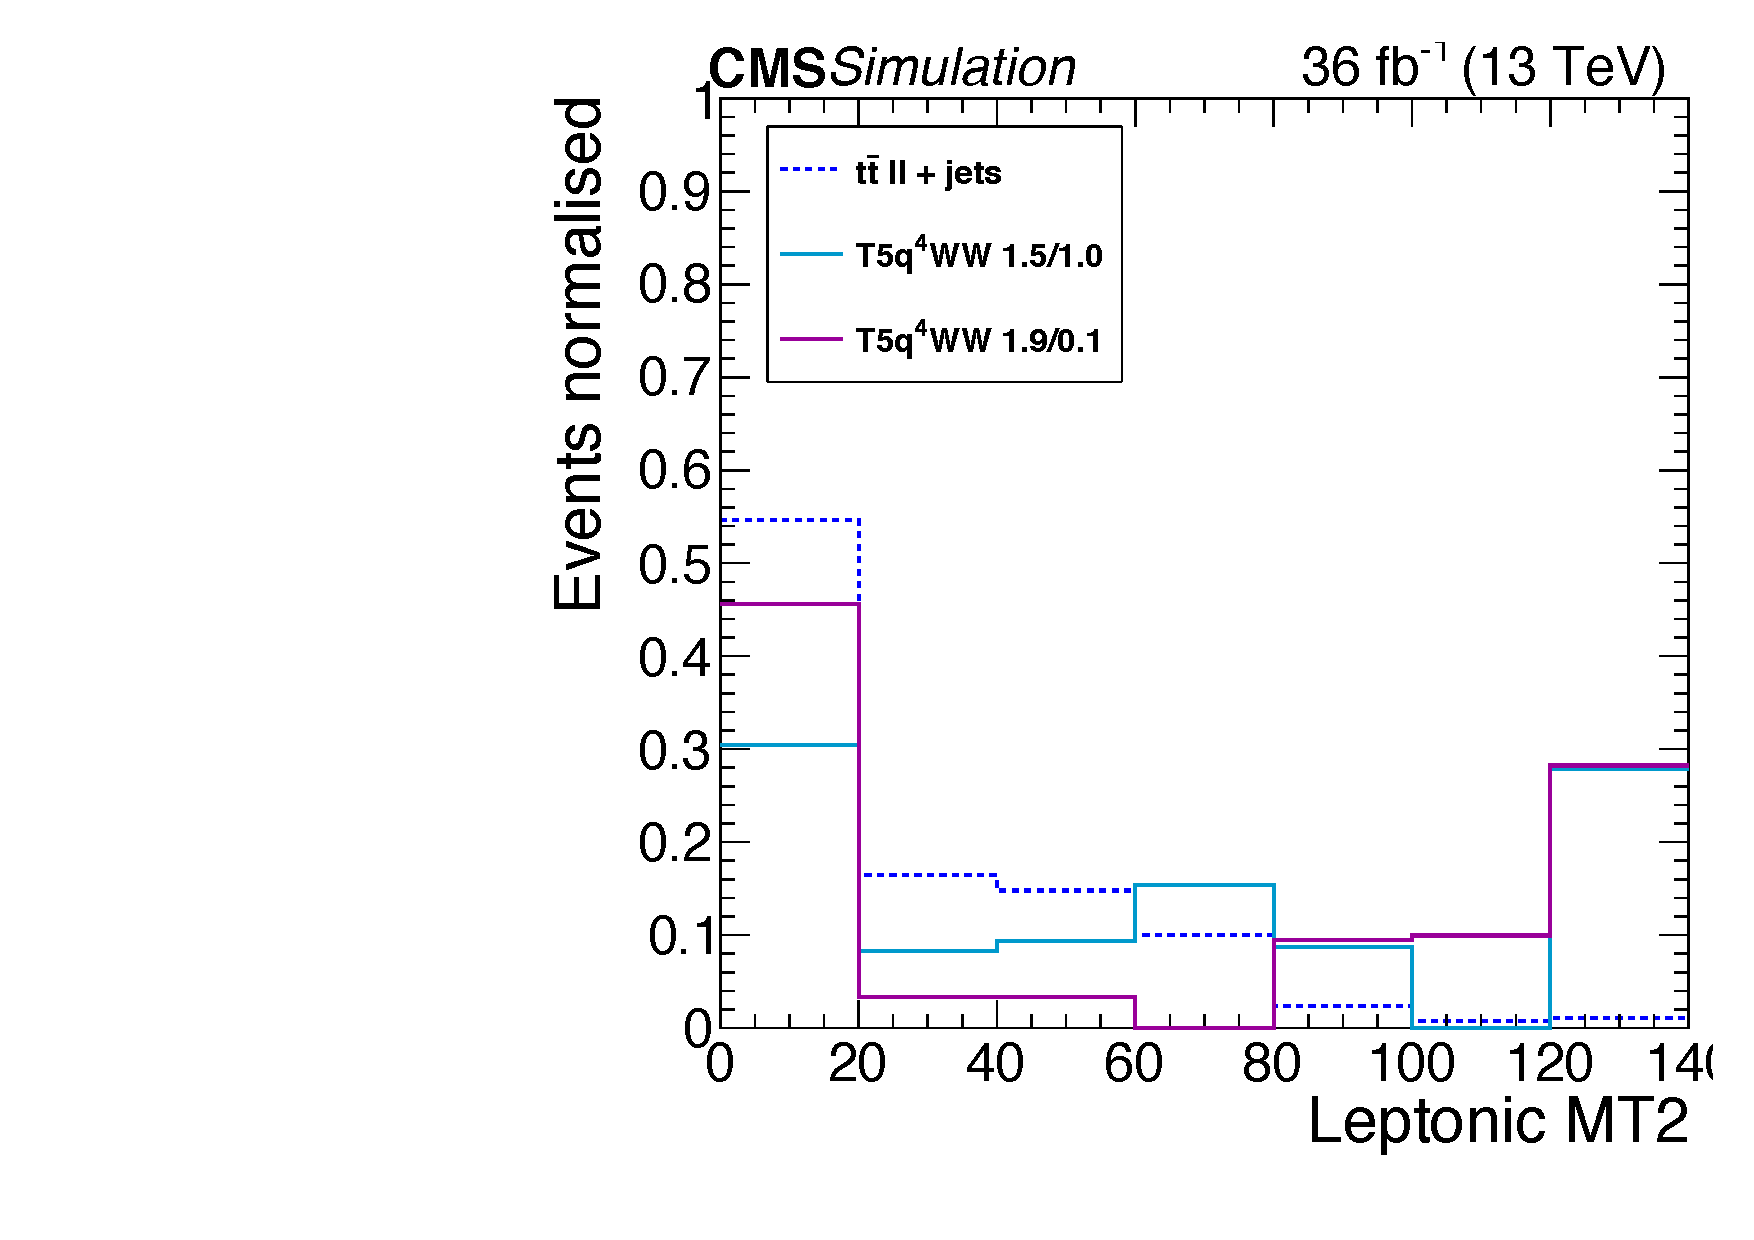
\includegraphics[width=0.3
    \textwidth]{Plots/analysis/isoveto/Mt2_nobReq_LEP.pdf}}
    \subfigure[\MTt\, with hadronic tracks]{ 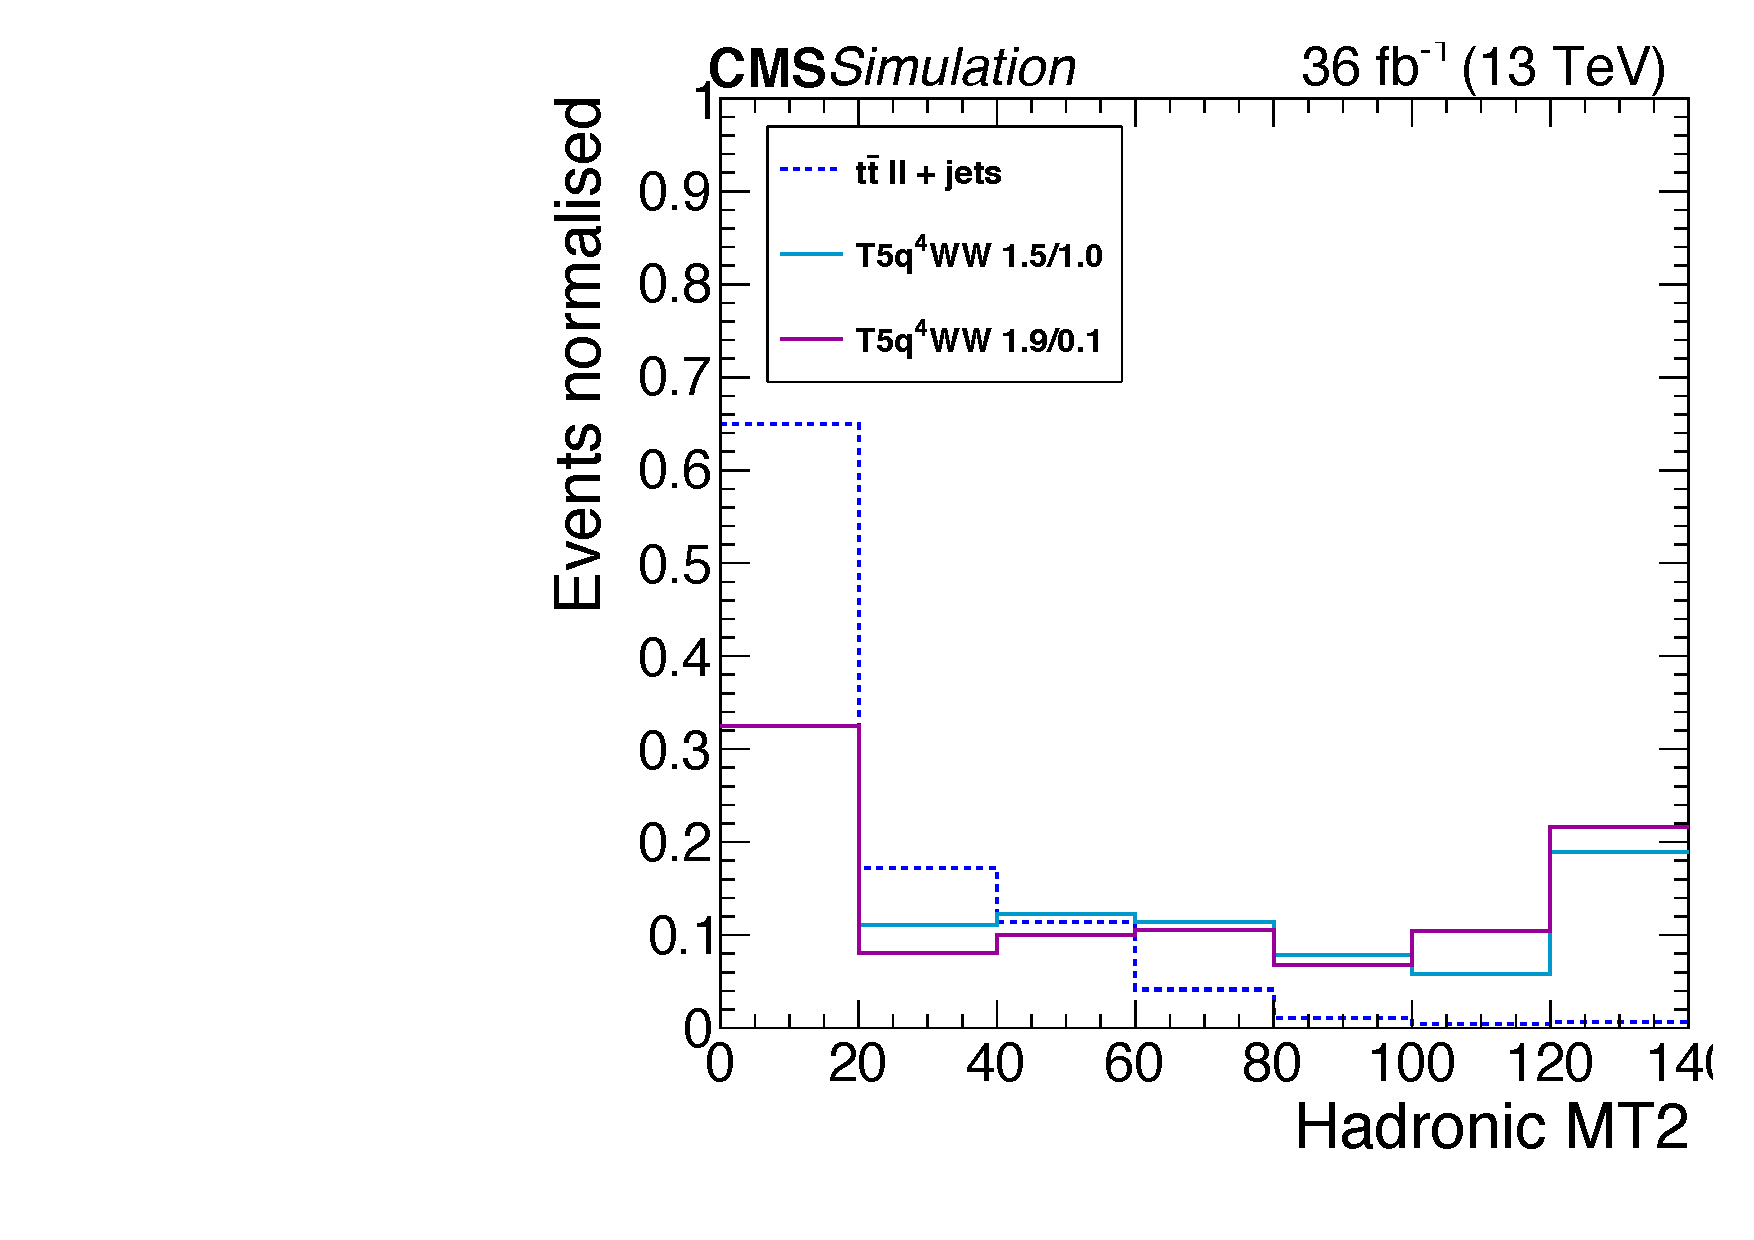
\includegraphics[width=0.3
    \textwidth]{Plots/analysis/isoveto/Mt2_nobReq_HAD.pdf}}
    \subfigure[\MTt\, (All events)        ]{ 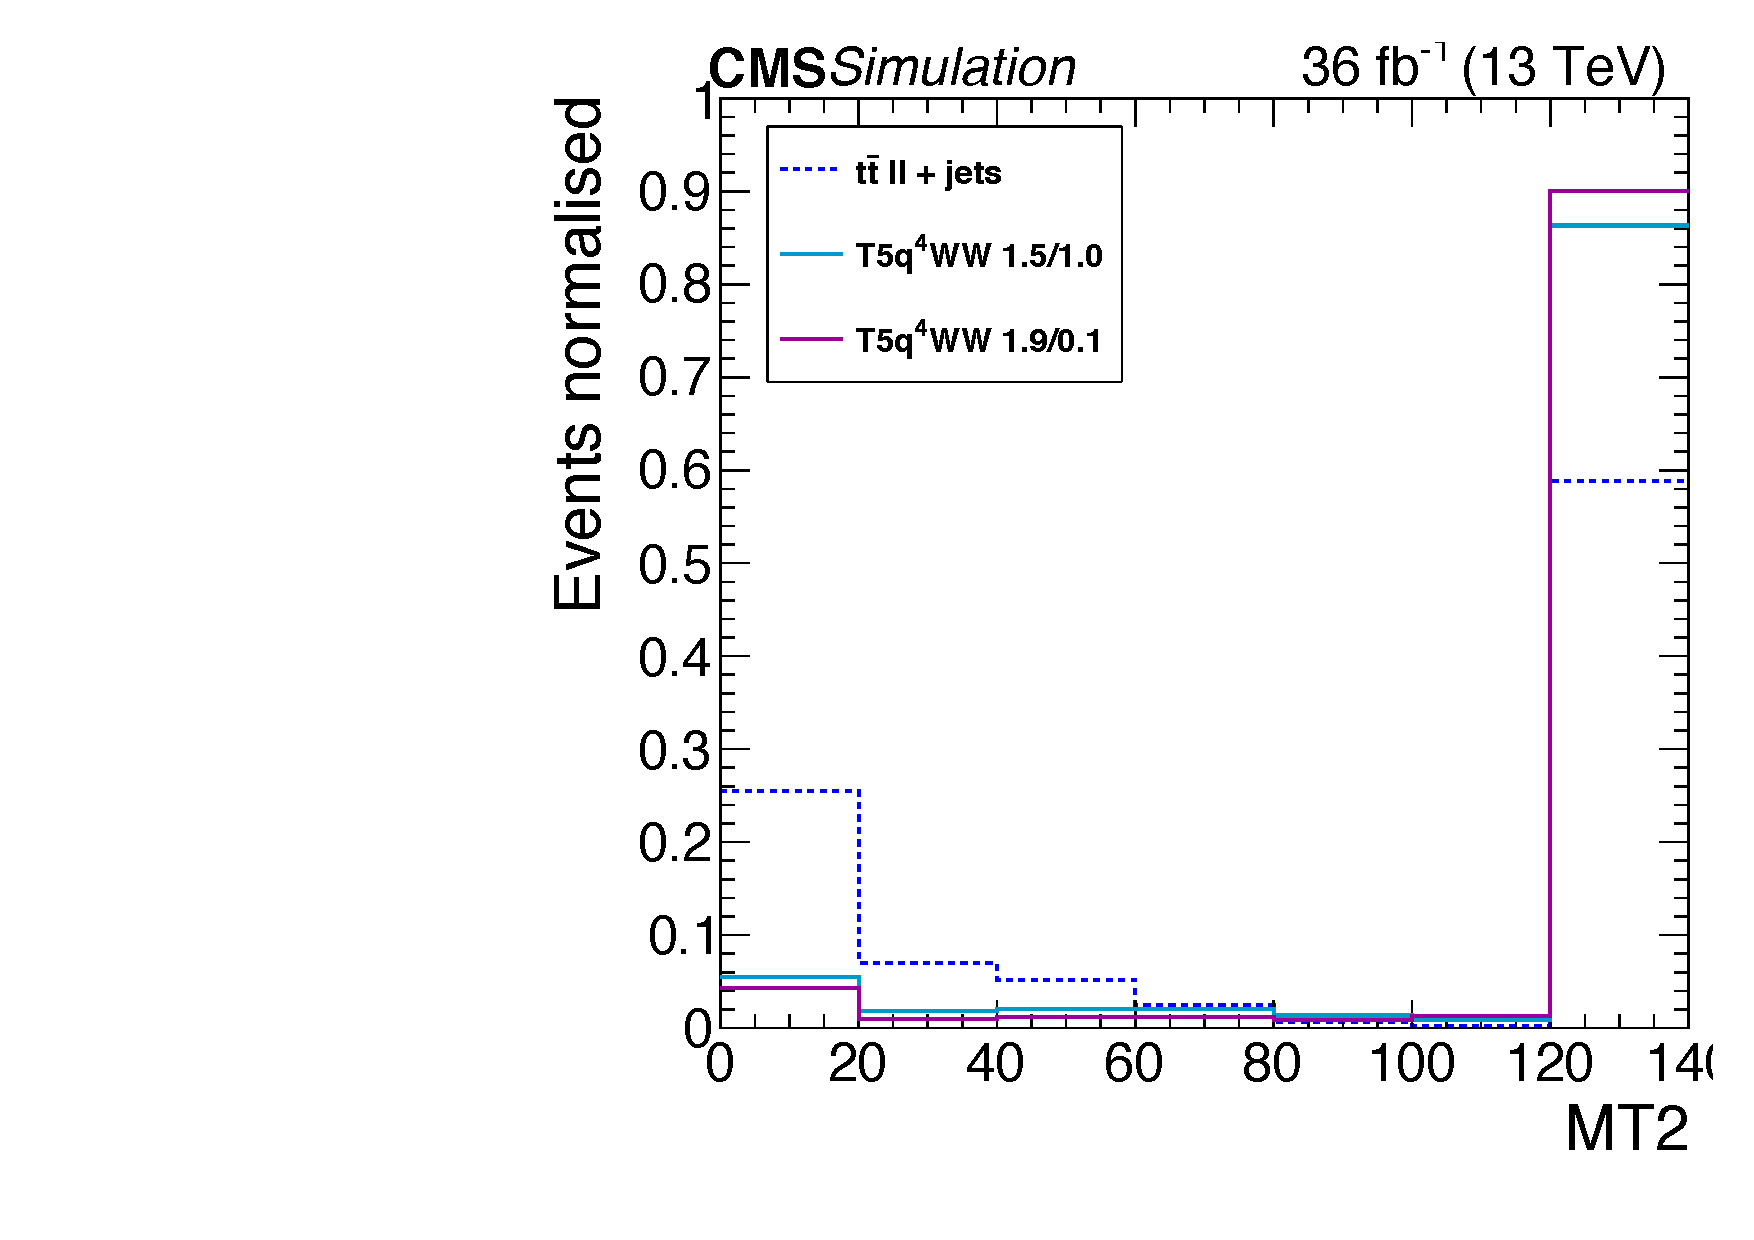
\includegraphics[width=0.3
    \textwidth]{Plots/analysis/isoveto/Mt2_nobReq_ALL.pdf}}
  \caption[Distributions of $\MTt$]{ \label{fig:track_mt2} Distributions of $\MTt$ for events with electron or muon veto tracks (a) and hadronic veto tracks (b), for dileptonic $\ttbar$ (blue dotted) and T5qqqqWW (purple and azure) signal samples. The highest bin is always an overflow bin. The majority $\ttbar$ events have $\MTt < 80$ GeV, while the signal events have longer tails in $\MTt$. The rightmost plot (c) shows the distribution for all events. 
  }
   \end{center}
\end{figure*}
\\
The effect of each baseline requirement is demonstrated in Fig.~\ref{fig:plotFlow} for the different background processes (stacked) and for two signal benchmark points, starting with a selection $\HT > 350$ GeV and $\LT > 150$ GeV. After this selection, the cuts are applied consecutively and the $\njet$ requirement has the biggest impact. It can be also noted that, naturally, the QCD background almost vanishes after the single muon selection. The estimation of important backgrounds will be explained in the Ch.~\ref{chap:Rcs}.
\renewcommand{\arraystretch}{1.5}
\begin{table}[ht]
\begin{center}
\caption{List of baseline criteria and object requirements.}\label{tab:CutSummary}
\begin{tabular}{|c|c|}\hline
Selection        & Definitions \\
\hline
\hline
Single lepton &Tight leptons, $\pt \geq 25$ GeV and $|\eta| < 2.4$\\
                      & and $I_{mini}<0.1(0.2)$ for electrons(muons)\\\hline
Lepton veto & Loose leptons, $\pt \geq 10$ GeV and $|\eta| < 2.4$ \\
		& and $I_{mini}<0.4$ \\\hline
Isolated track veto & $I_{rel}<0.3$, $\Delta R(\ell,{\rm t}) <0.1$, ${\rm t}_{\rm charge}$ = -${l}_{\rm charge}$  \\\hline
$n_{jets} \geq 5$ & Jets with $\pt \geq 30$ GeV and $|\eta| < 2.4$ \\
\cline{1-1}
$p_{T,jets\,(1,2)} \geq 80$ GeV & and cleaned from close leptons \\\hline
$H_T \geq 500$ GeV & $\sum_{jets} \pt$\\\hline
$L_T \geq 250$ GeV &  $\MET + \pt^{lep}$ \\\hline
$n_{b-tag} = 0$ & b-tagged jets with CSVv2 Medium working point (0.8484)\\\hline
\end{tabular}
\end{center}
\end{table}
\renewcommand{\arraystretch}{1}
 \begin{figure*}[!hbt]
    \begin{center}
    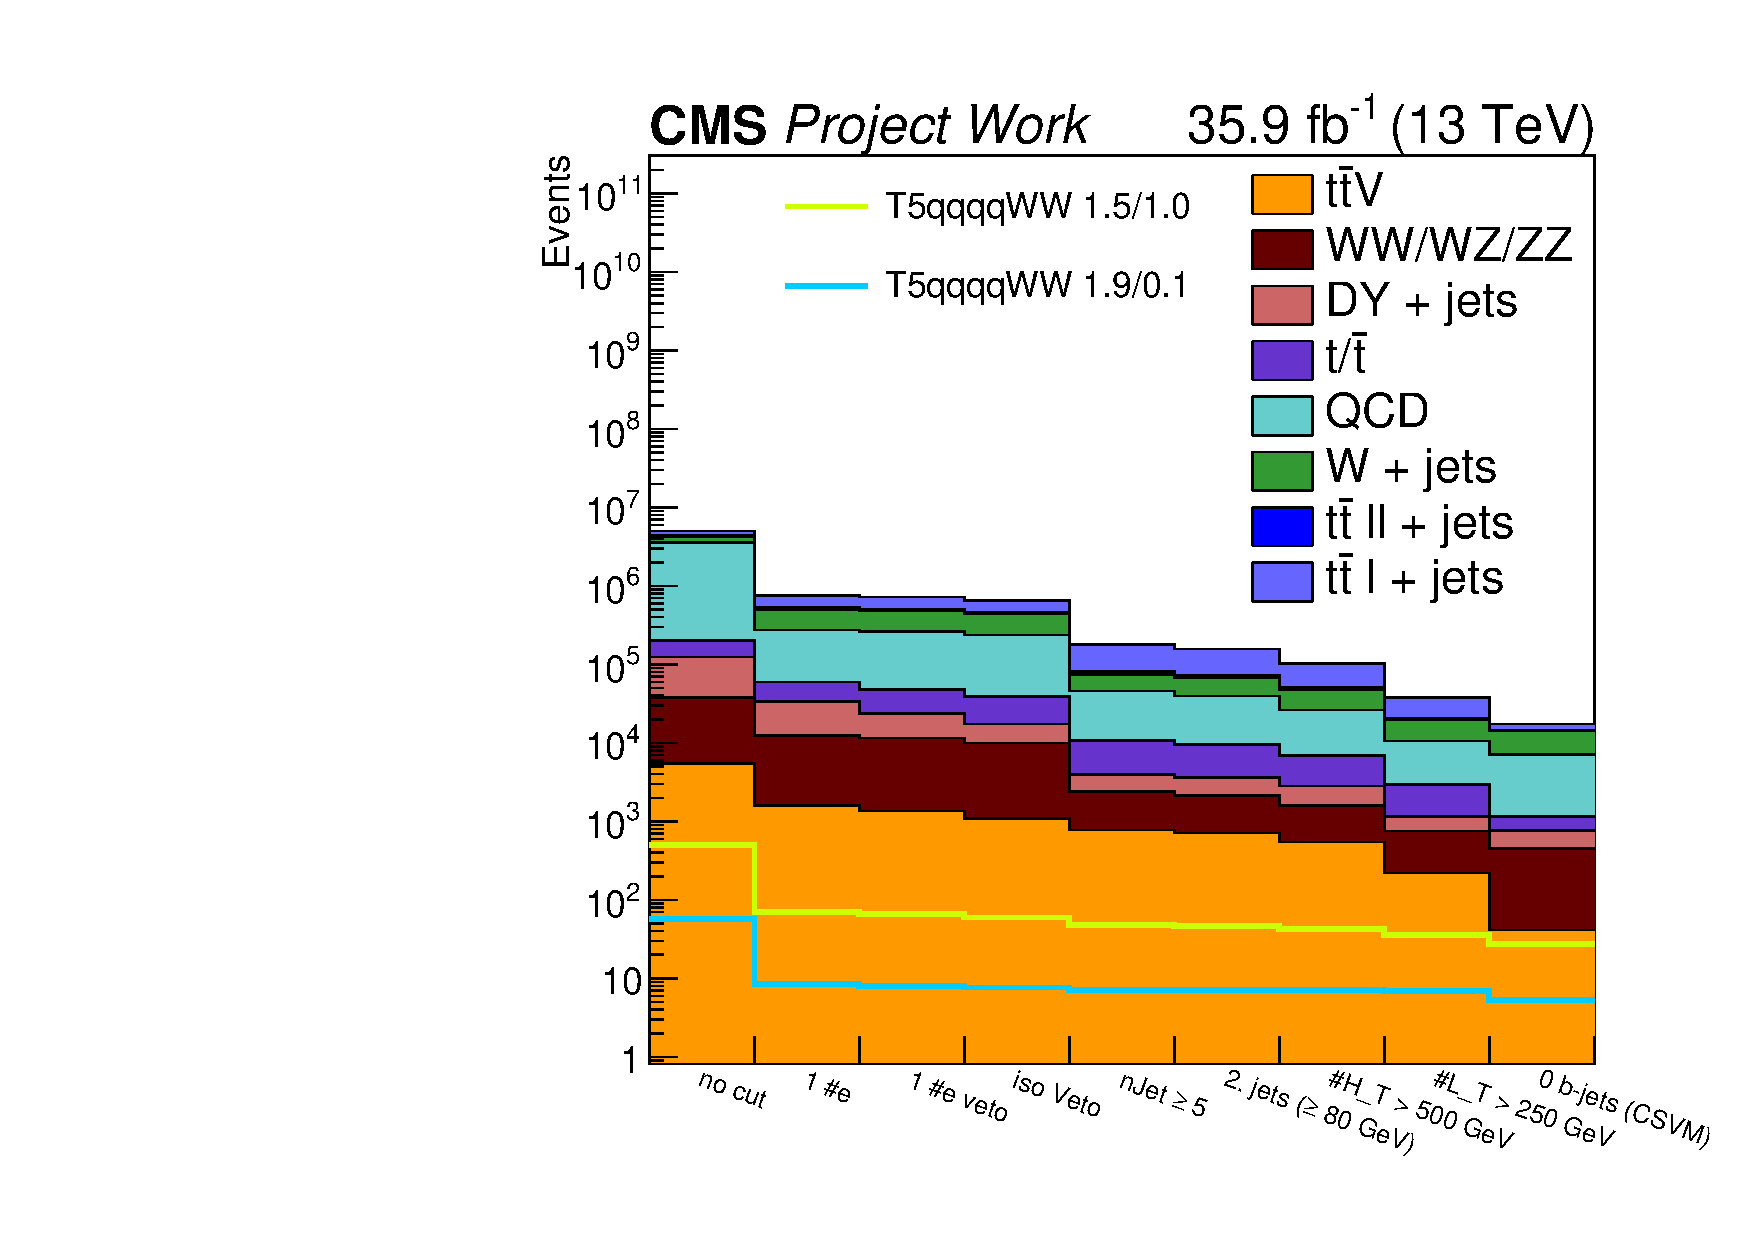
\includegraphics[width=0.45\textwidth]{Plots/analysis/cutflow/electron}
     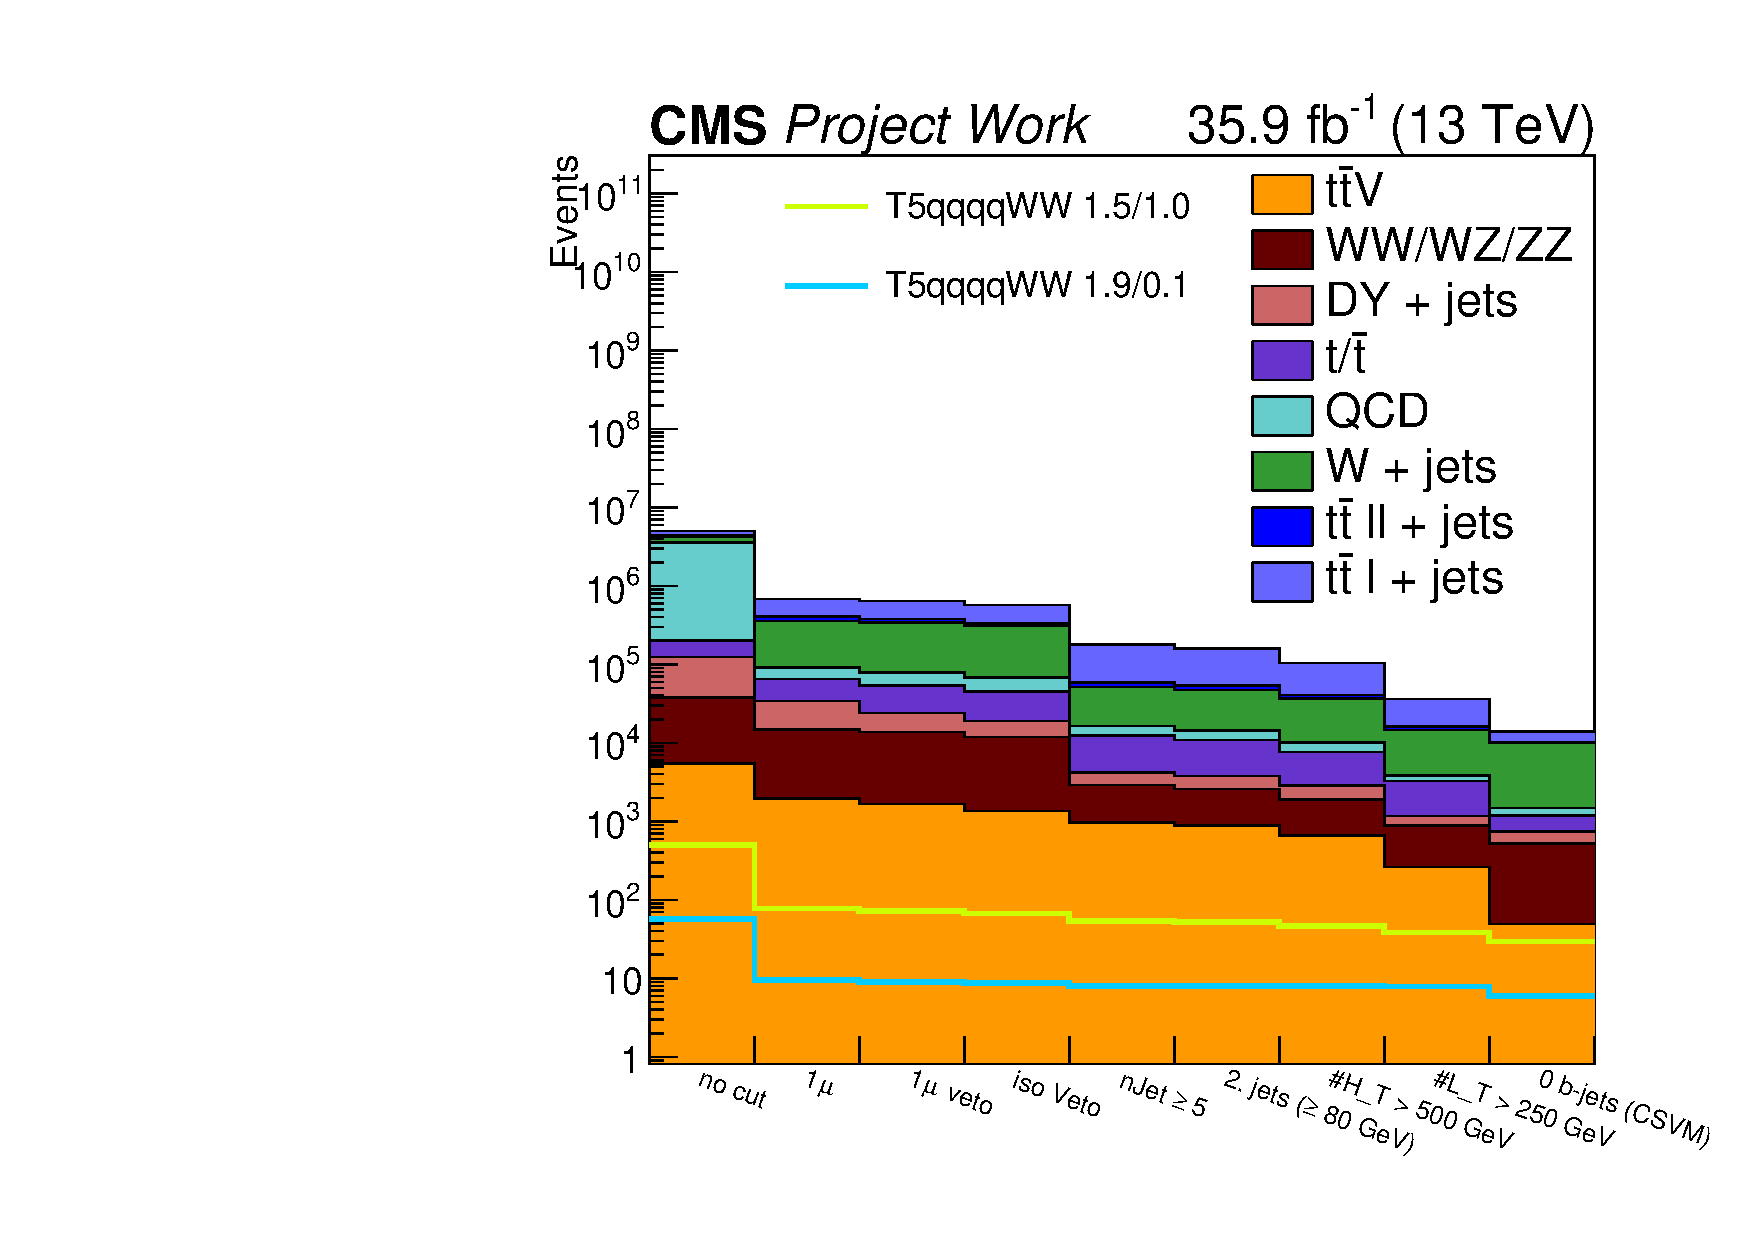
\includegraphics[width=0.45\textwidth]{Plots/analysis/cutflow/muon}
  \caption{ \label{fig:plotFlow} The selection criteria flow for the electron (left) and muon (right) channel. Samples are scaled to the luminosity with their cross section and scale factors discussed in Sec.~\ref{sec:SF}.
  }
   \end{center}
\end{figure*}
\newpage
\section{Data samples}
In this work, the data recorded by the CMS detector during the 2016 LHC run at 13 TeV is used. As shown in Fig.~\ref{fig:peaklumi_IntLumi}~(right), the total integrated luminosity collected by CMS is 37.76 fb$^{-1}$. The data validated according to the CMS Data Quality Monitoring~(CMS-DQM) certification requirements is L=35.9~fb$^{-1}$.
\subsection{Trigger selection}
\label{sec:triggers}
Most events in this work are selected by a combination of triggers requiring an isolated single lepton, electron or muon, with $\pt$ of 15~GeV and $\HT$ of 350~GeV. 
%To recover inefficiencies due to an update on the online electron ID and the saturated L1-jets, the trigger strategy had to be extended: 
The complete list of trigger paths can be found in Tab.~\ref{tab:triggers}. The naming of the trigger paths relates to the conditions introduced on the corresponding object. For example, HLT\_Ele105\_CaloIdVT\_GsfTrkIdT involves the conditions that the electron has $\pt$ larger than 105~GeV and it satisfies the very tight calorimeter identification and the tight GSF identification.\\
\renewcommand{\arraystretch}{1.5}
\begin{table}[!h]
\begin{center}
\caption{List of HLT paths. Notation is used in terms of CMS internal shortcuts.}\label{tab:triggers}
\resizebox{\columnwidth}{!}{
\begin{tabular}{|c|}\hline
Single Electron dataset \\
\hline
\hline
      HLT\_Ele105\_CaloIdVT\_GsfTrkIdT \\
      HLT\_Ele115\_CaloIdVT\_GsfTrkIdT \\
      HLT\_Ele50\_CaloIdVT\_GsfTrkIdT\_PFJet165\\
      HLT\_Ele27\_WPTight\_Gsf \\
      HLT\_Ele15\_IsoVVVL\_PFHT350 \\
      HLT\_Ele15\_IsoVVVL\_PFHT400 \\
\hline
Single Muon dataset \\
\hline
\hline
      HLT\_Mu50 \\
      HLT\_IsoMu24\\
      HLT\_IsoTkMu24\\
      HLT\_Mu15\_IsoVVVL\_PFHT350 \\
      HLT\_Mu15\_IsoVVVL\_PFHT400\\
\hline
MET dataset \\
\hline
\hline
      HLT\_PFMET100\_PFMHT100\_IDTight OR  HLT\_PFMETNoMu100\_PFMHTNoMu100\_IDTight \\
      HLT\_PFMET110\_PFMHT110\_IDTight OR  HLT\_PFMETNoMu110\_PFMHTNoMu110\_IDTight \\
      HLT\_PFMET120\_PFMHT120\_IDTight OR HLT\_PFMETNoMu120\_PFMHTNoMu120\_IDTight  \\
\hline
\end{tabular}}
\end{center}
\end{table}
\renewcommand{\arraystretch}{1}
Events recorded with these trigger paths are allocated in three primary datasets~(PDs): the \textbf{SingleElectron}, \textbf{SingleMuon} and \textbf{MET} datasets.
Therefore, when successively adding PDs, triggers contained in previous PDs are vetoed to avoid double counting of events contained in more than one of the PDs. The trigger efficiency calculation is shown in Eq.~\ref{Eqtrig}. The trigger efficiencies are measured as a function of $\LT$, $\HT$ and lepton $\pt$ and can be seen in Figs.~\ref{fig:trig_eff_LT},~\ref{fig:trig_eff_HT},~\ref{fig:trig_eff_leptonPt} respectively.
The efficiency in the baseline region (\LT$>$250 GeV; \HT$>$500 GeV; lepton $\pt$ $>$25 GeV) is flat and its value is close to 100\%(98\%) for the muons (electrons).
\begin{equation}
\label{Eqtrig}
  \epsilon = \frac{N({\rm all \; events \; passing \; probed \; trigger(s) +
  preselection + reference \; trigger})}{N({\rm all \; events \; passing
  \;preselection + reference \; trigger})}
\end{equation}
\begin{figure*}[!h]
  \begin{center}
    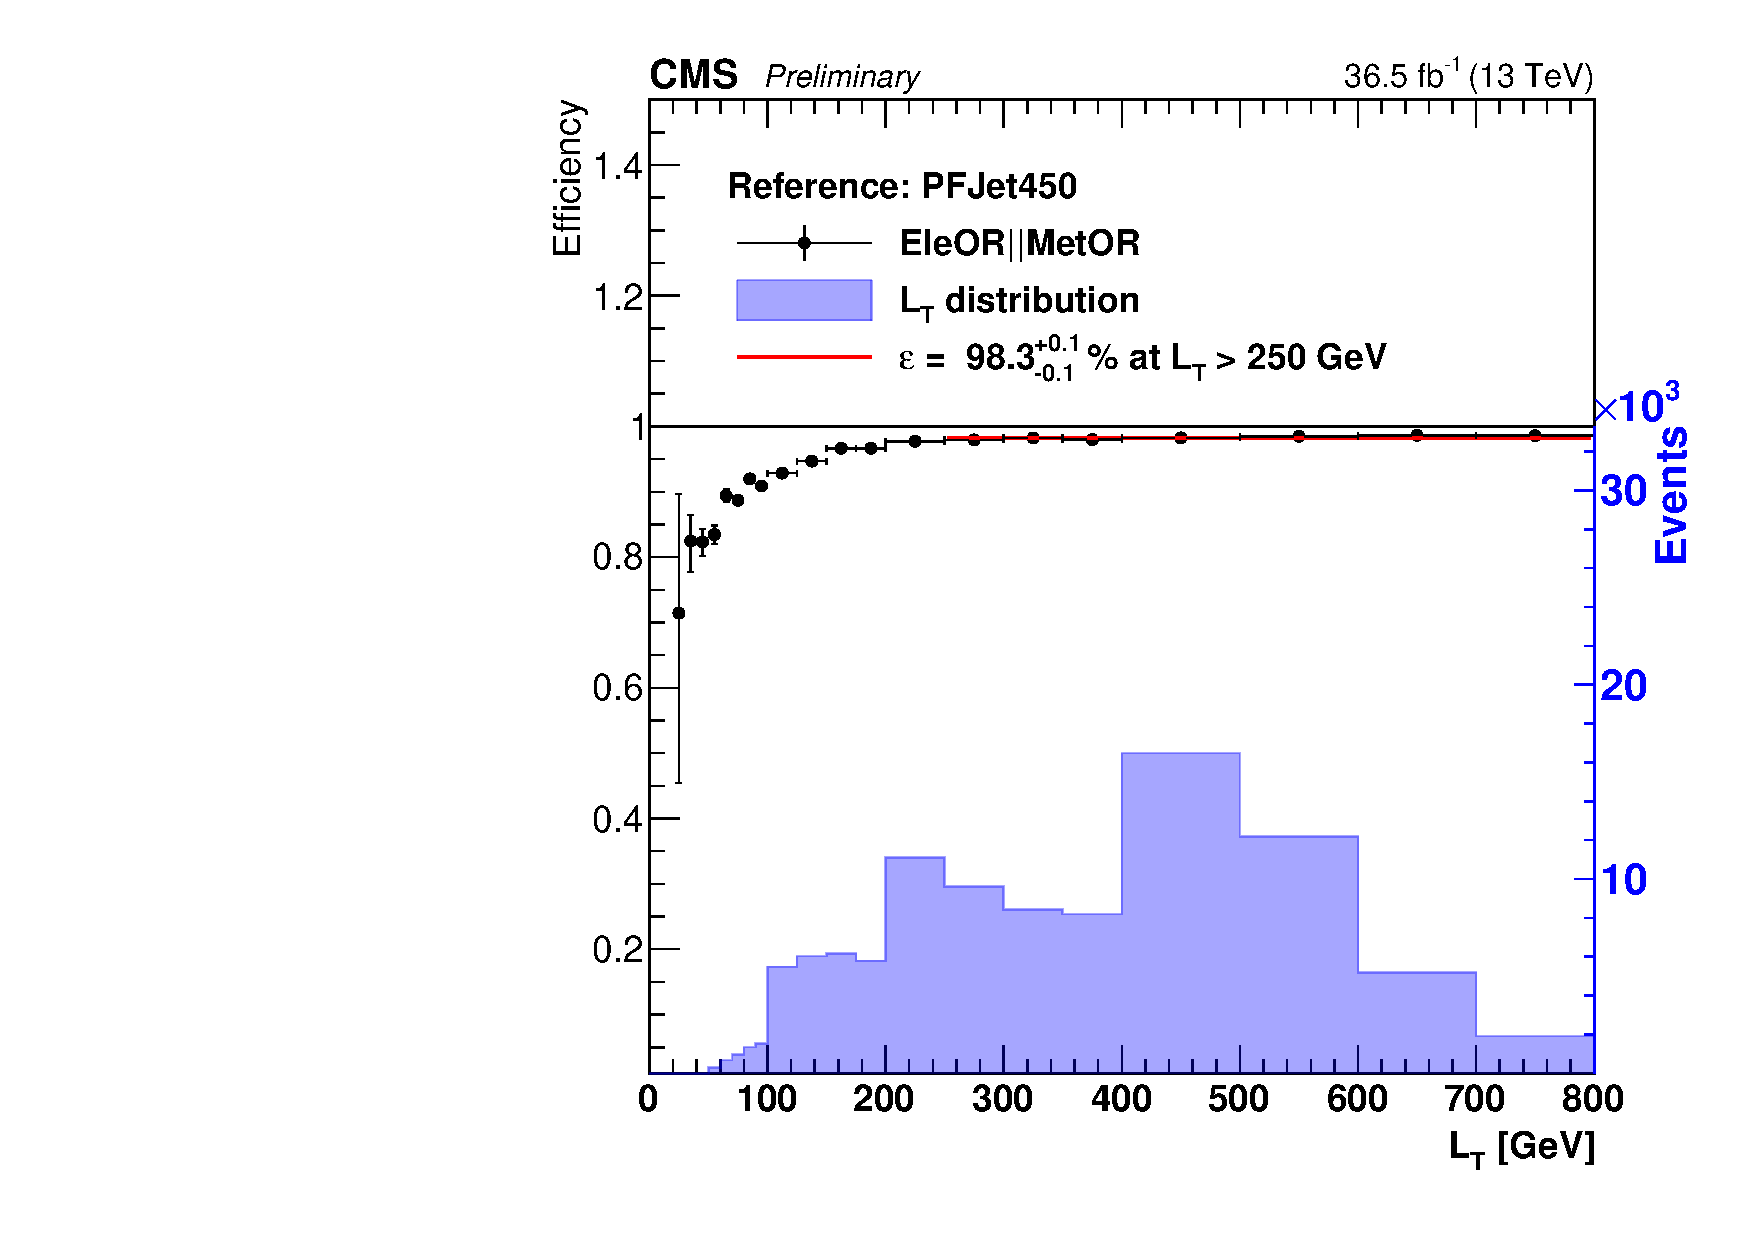
\includegraphics[width=0.45\textwidth]{Plots/trigger/LT_PFJet450_EffFit_test_HLT_EleORORHLT_MetOR.pdf}
    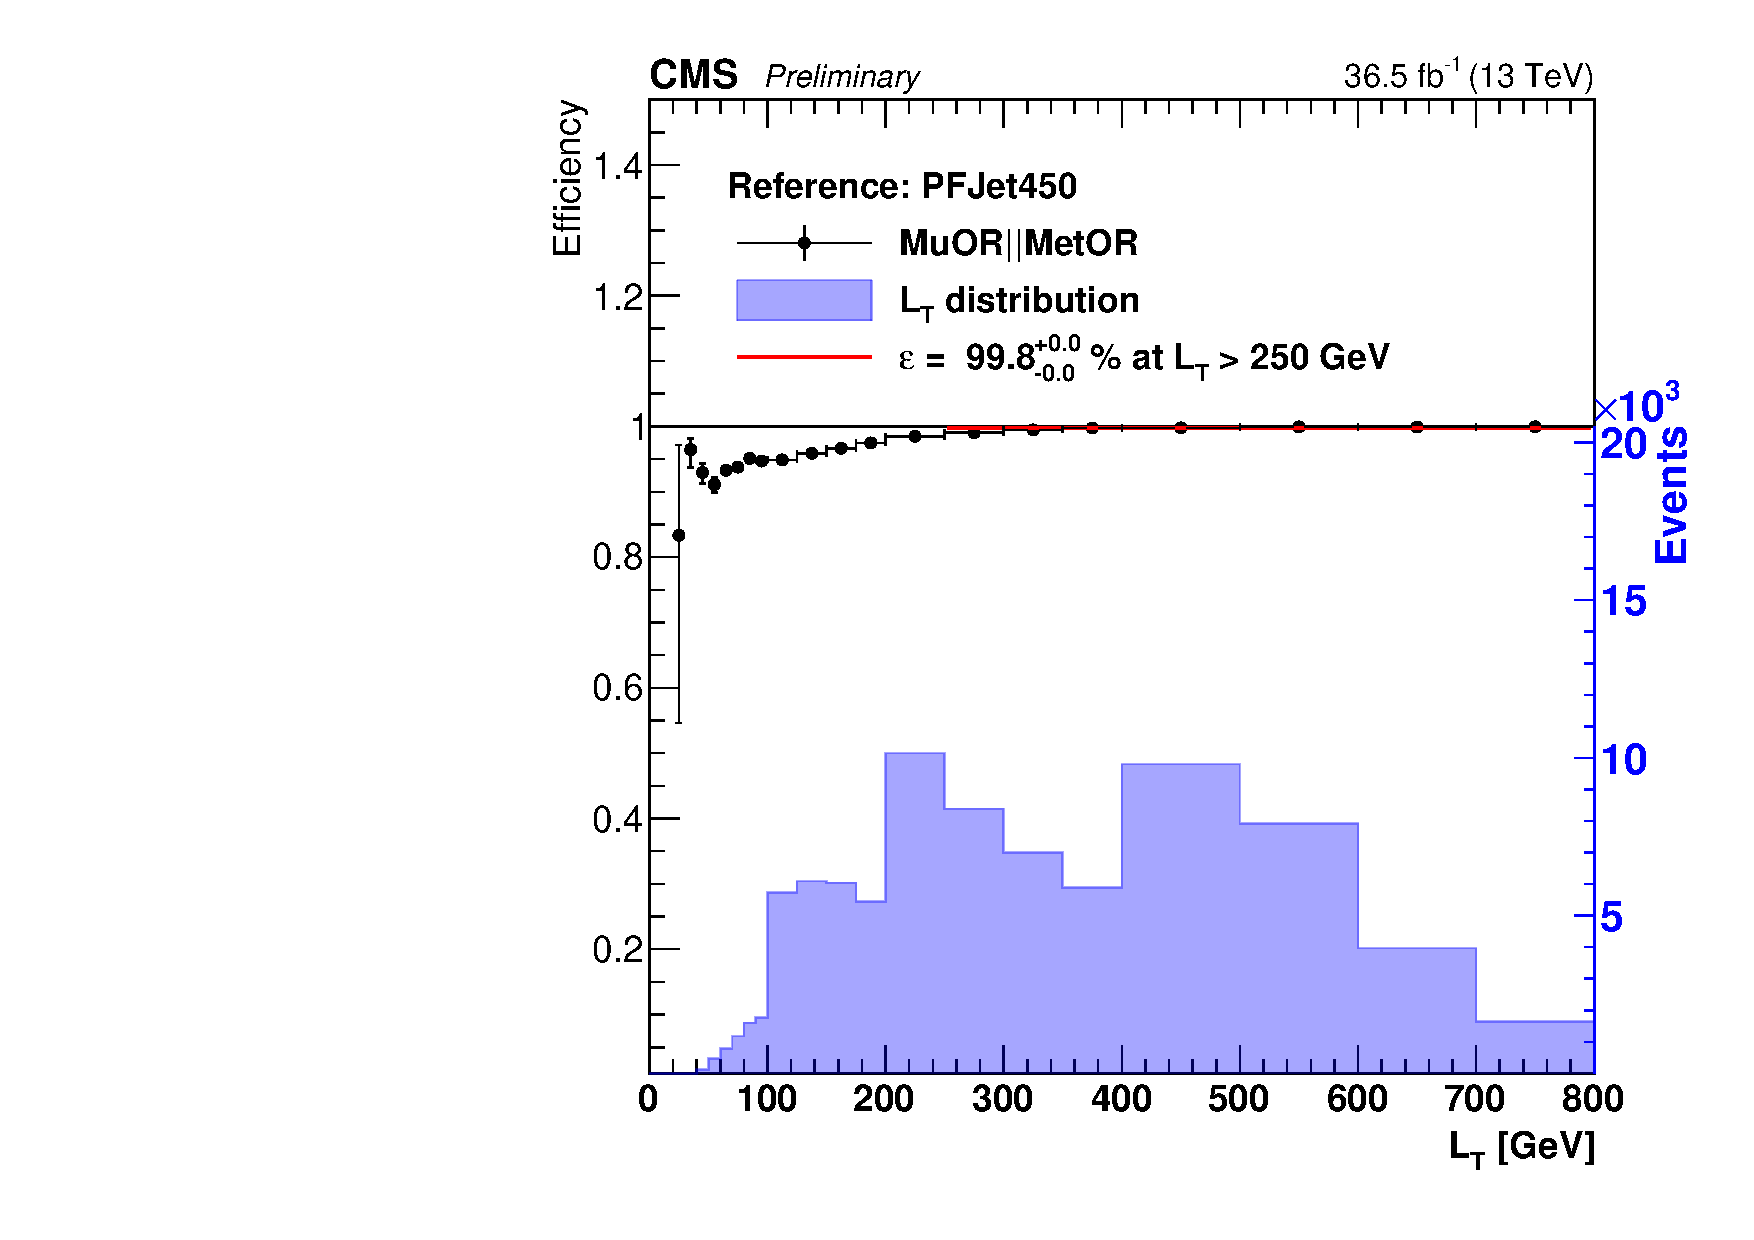
\includegraphics[width=0.45\textwidth]{Plots/trigger/LT_PFJet450_EffFit_test_HLT_MuORORHLT_MetOR.pdf}
  \end{center}
  \caption[The trigger efficiency as a function of $\LT$]{Measurement of the trigger efficiency as a function of $\LT$ for the electron trigger selection (see Tab.~\ref{tab:triggers}) on the right~\cite{trigger}.
    %The number of events passing the trigger selection is given as shaded
    %histogram
  \label{fig:trig_eff_LT}}
  \end{figure*}
\begin{figure*}[!h]
  \begin{center}
    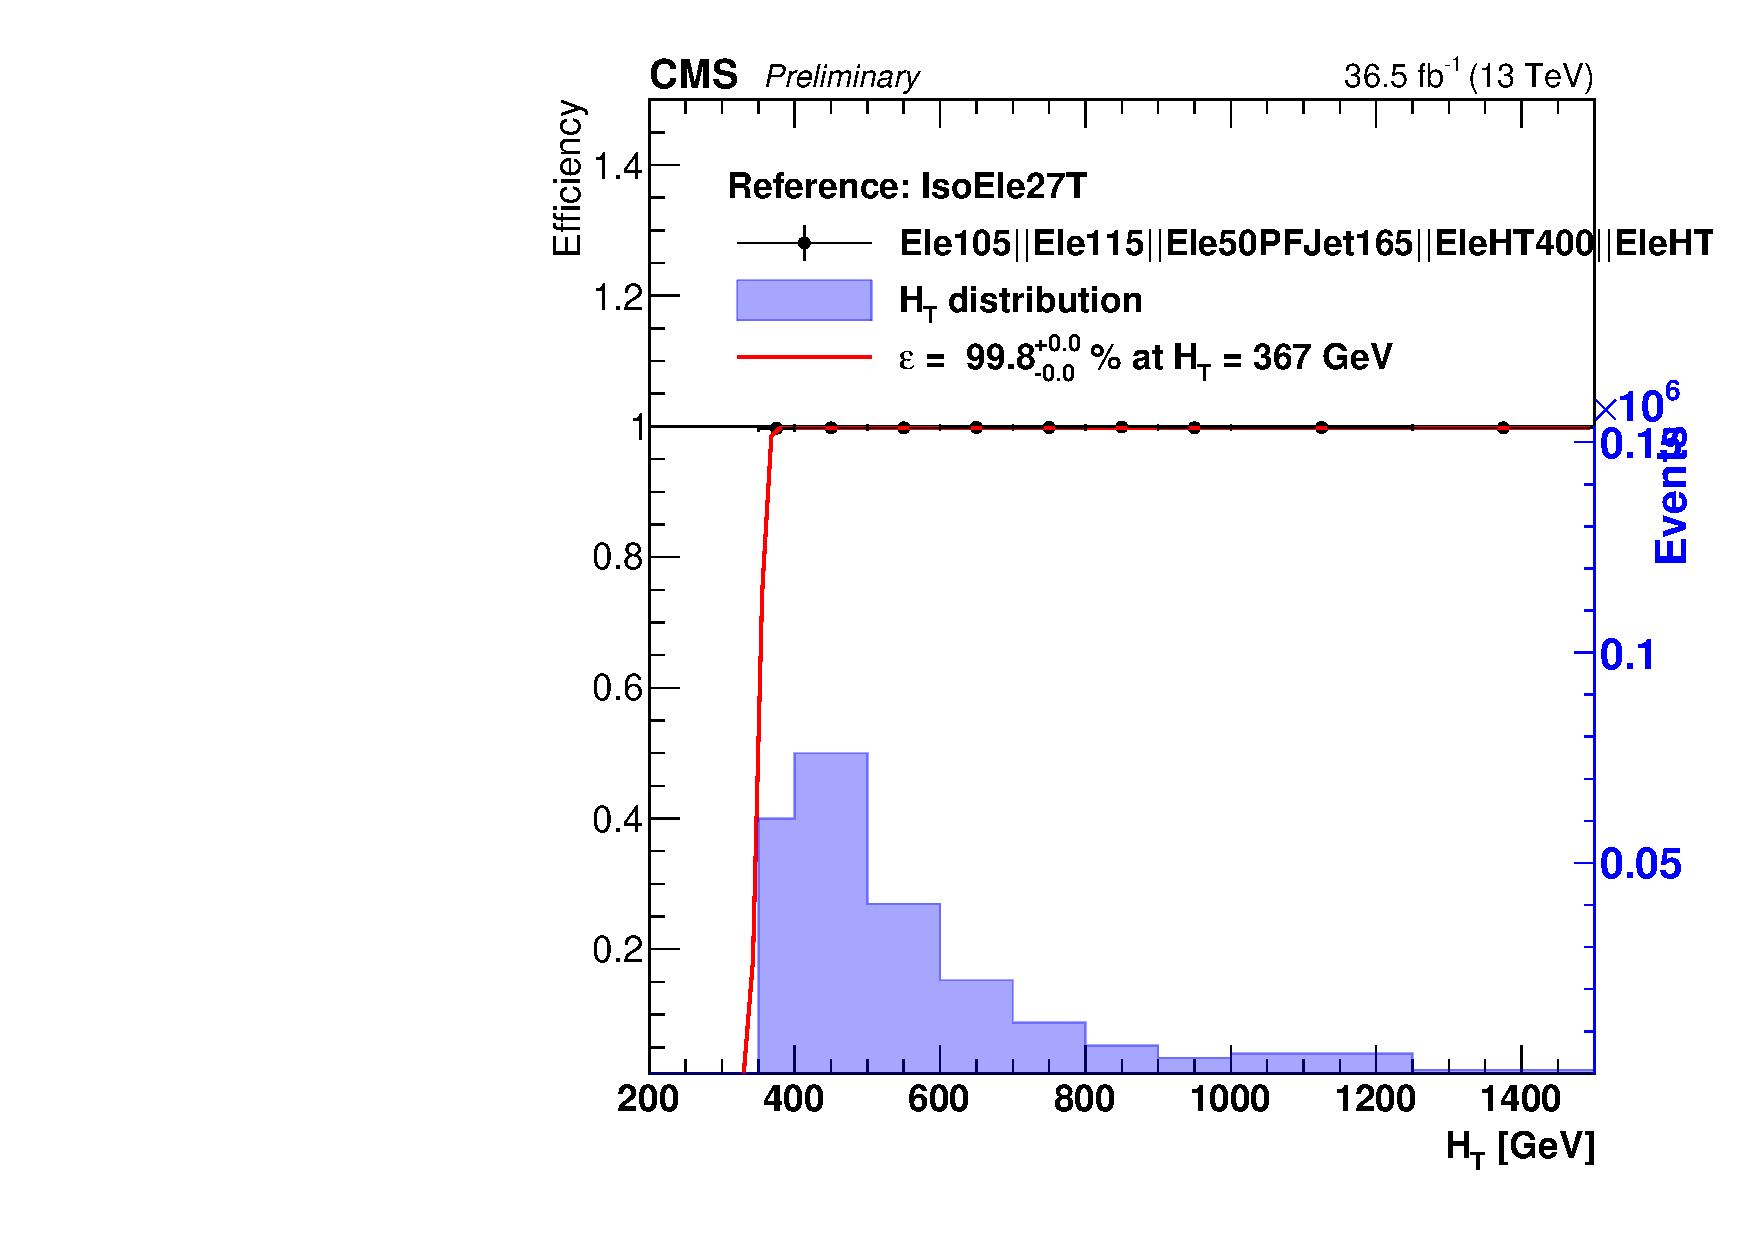
\includegraphics[width=0.45\textwidth]{Plots/trigger/HT_IsoEle27T_EffFit_test_HLT_Ele105ORHLT_Ele115ORHLT_Ele50PFJet165ORHLT_EleHT400ORHLT_EleHT350ORHLT_MetOR.pdf}
    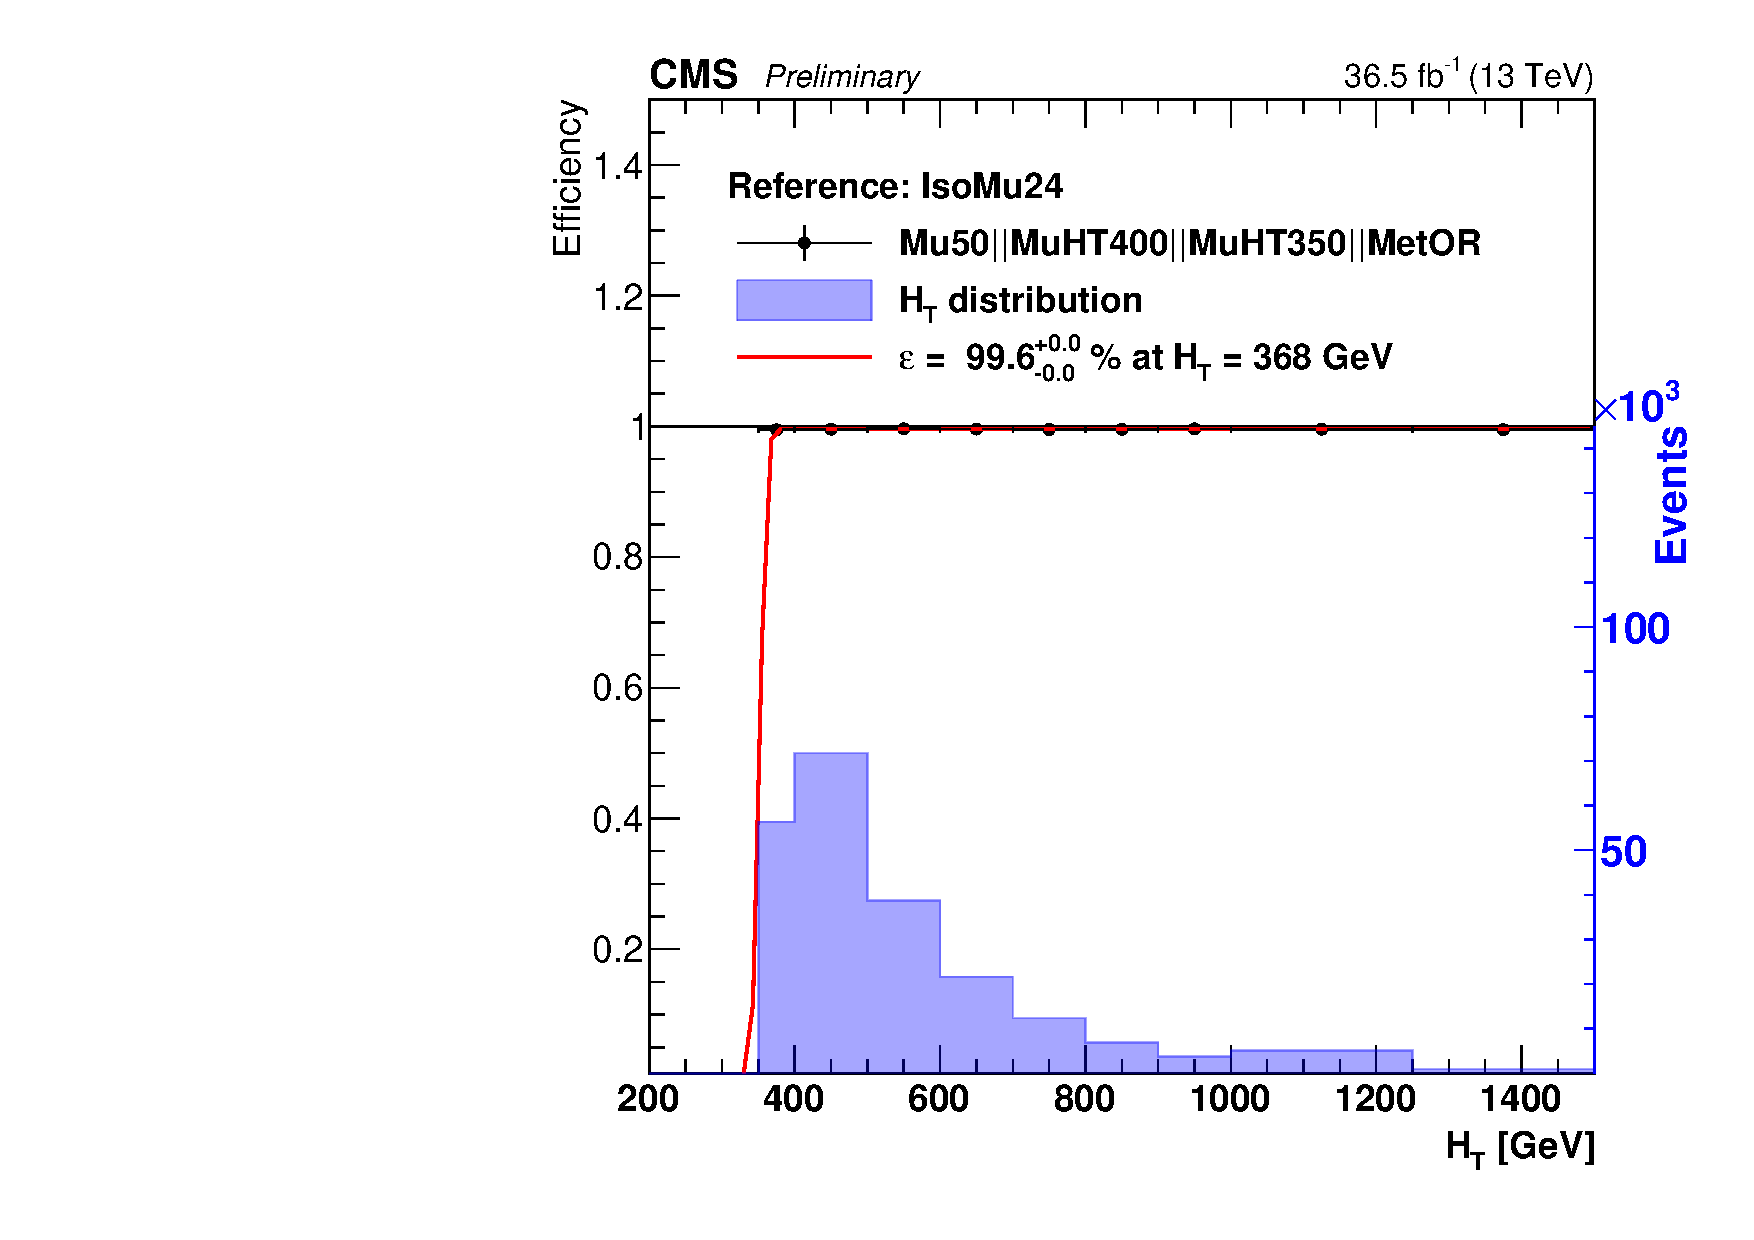
\includegraphics[width=0.45\textwidth]{Plots/trigger/HT_IsoMu24_EffFit_test_HLT_Mu50ORHLT_MuHT400ORHLT_MuHT350ORHLT_MetOR.pdf}
  \end{center}
  \caption[The trigger efficiency as a function of $\HT$]{Measurement of the trigger efficiency as a function of $\HT$ for the electron trigger selection on the left and the muon trigger selection  on the right~\cite{trigger}.
    %The number of events passing the trigger selection is given as shaded
    %histogram
  \label{fig:trig_eff_HT}}
  \end{figure*}
  \begin{figure*}[!h]
    \begin{center}
    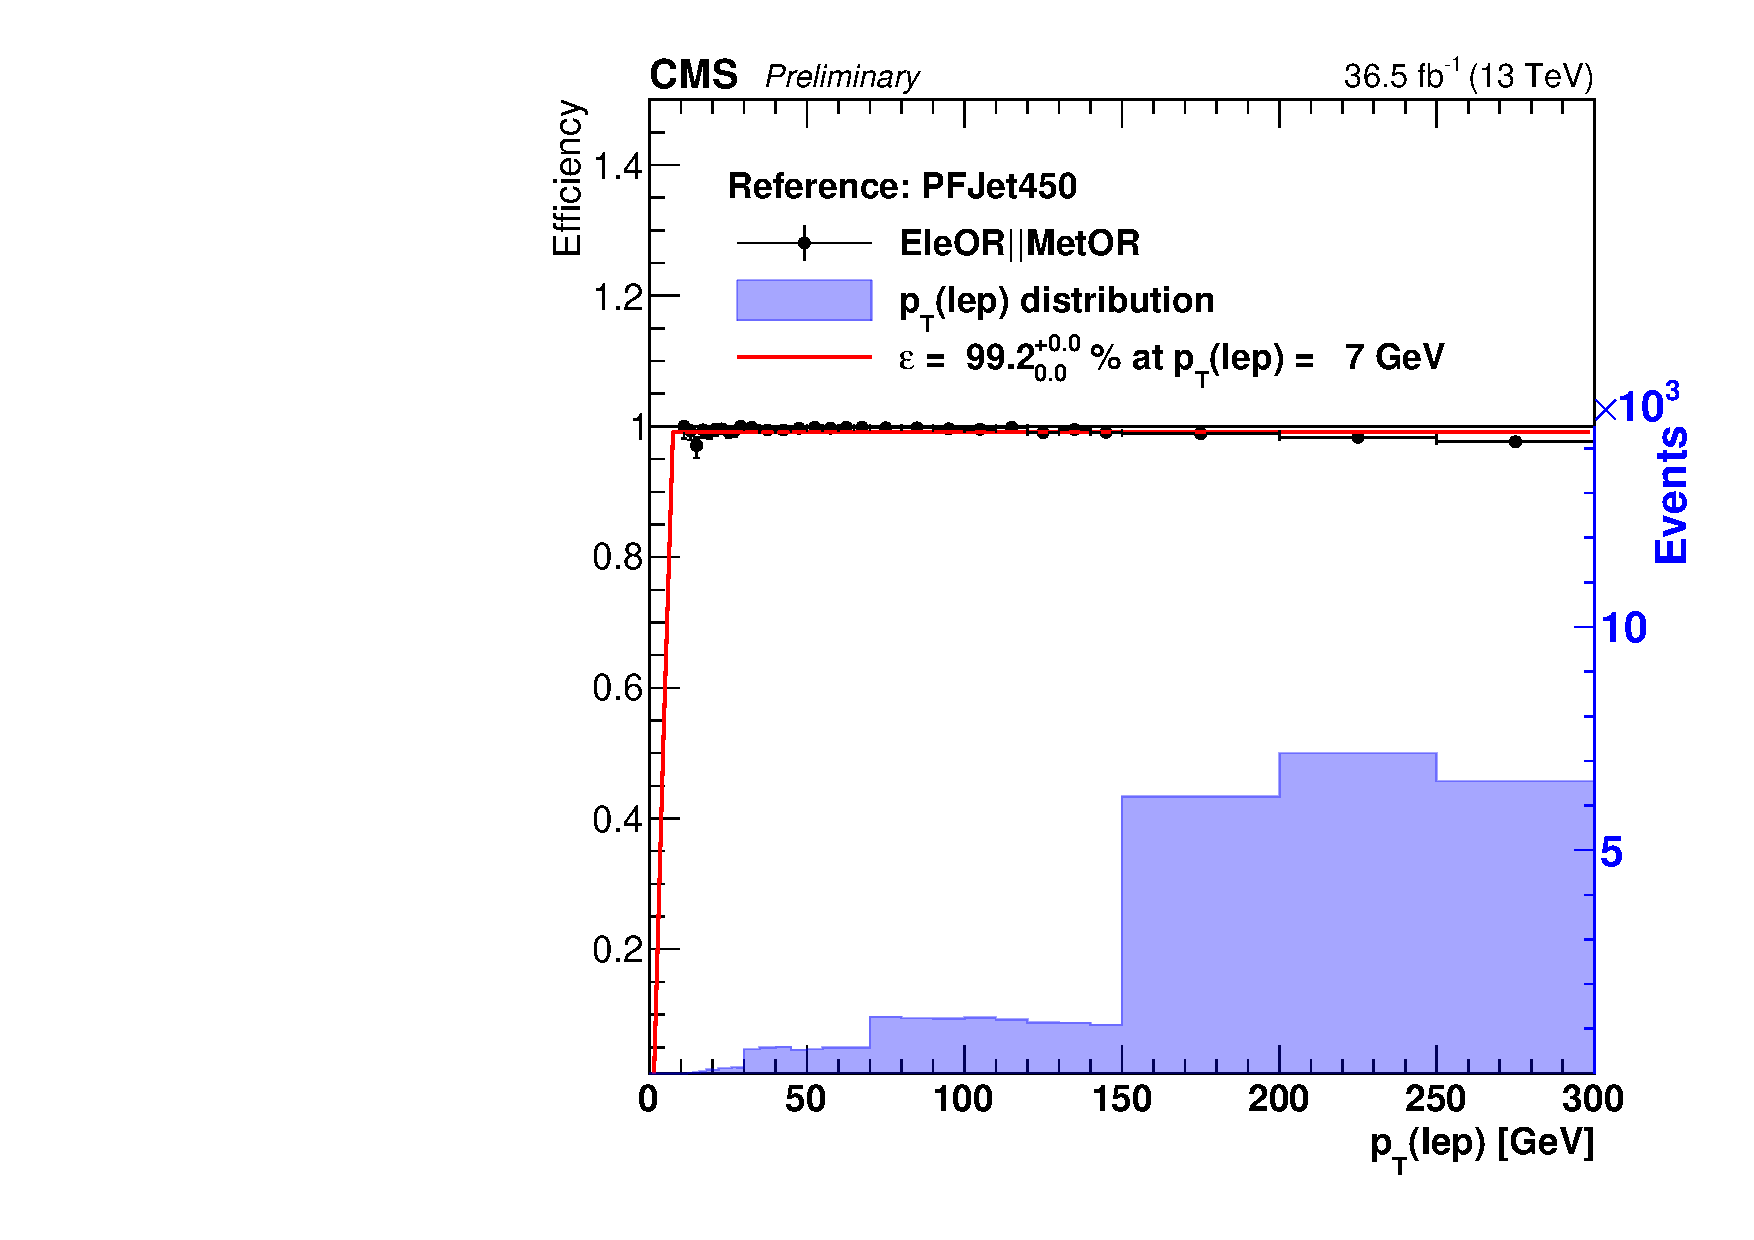
\includegraphics[width=0.45\textwidth]{Plots/trigger/LepPt_PFJet450_EffFit_test_HLT_EleORORHLT_MetOR.pdf}
    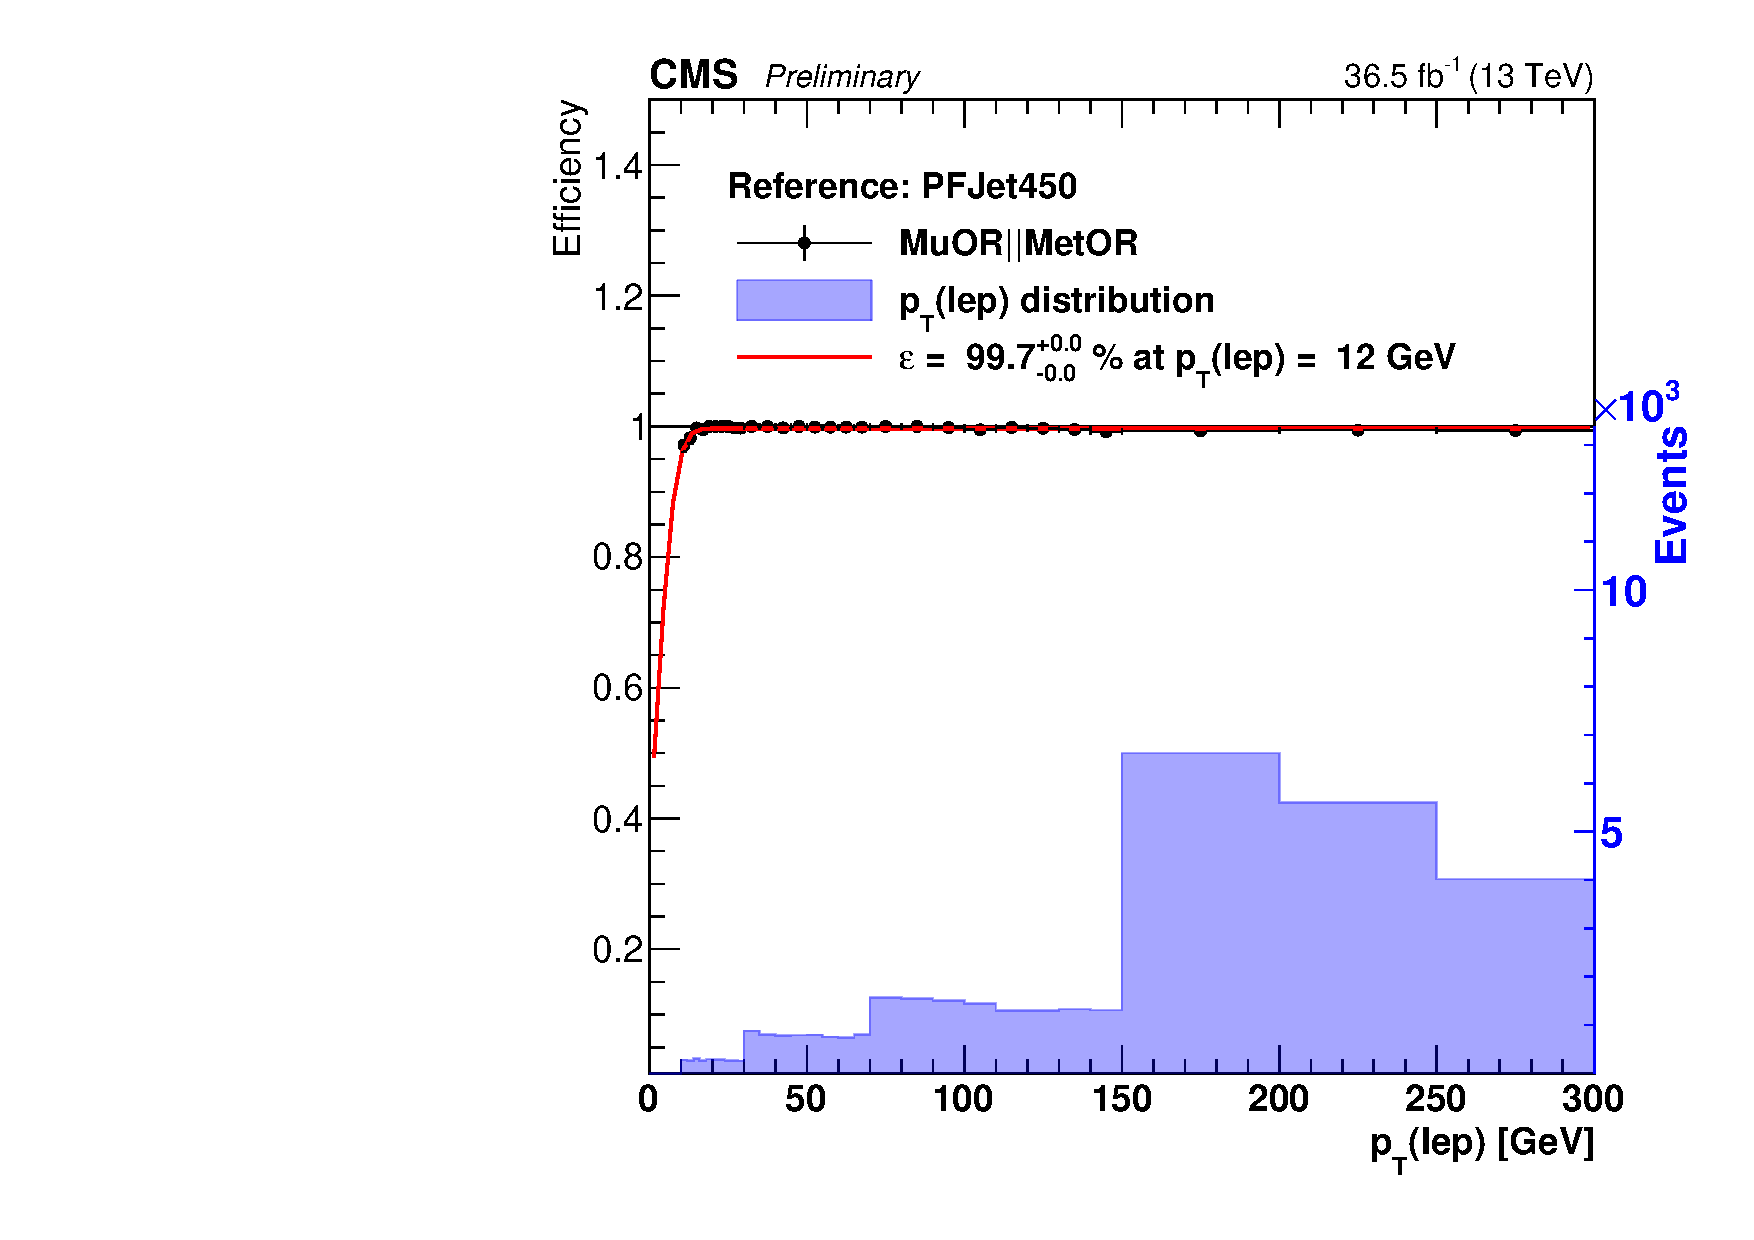
\includegraphics[width=0.45\textwidth]{Plots/trigger/LepPt_PFJet450_EffFit_test_HLT_MuORORHLT_MetOR.pdf}
  \end{center}
  \caption[The trigger efficiency as a function of lepton $\pt$]{Measurement of the trigger efficiency as a function of lepton $\pt$ for the
    electron trigger selection is shown on the left and the muon trigger selection is shown on the right. The lepton $\pt$ trigger efficiency is measured after an $\LT>250$~GeV requirement which is the analysis baseline selection~\cite{trigger}.
    %The number of events passing the trigger selection is given as shaded
    %histogram
  \label{fig:trig_eff_leptonPt}}
\end{figure*}
\newpage
\section{Event cleaning filters}
\label{sec:filters}
Spurious detector signals can produce artificially large $\MET$. Sources and dedicated algorithms that are used to identify and remove the events with fake $\MET$ are briefly discussed in the following.\\
%The event reconstruction can fail due to the noisy detector cells and other kinds of detector problems. These can result in incorrectly reconstructed physics objects such as: muons, jets and hence MET. In CMS, the physics object groups related to the problem release event filters or cures for the falsely reconstructed objects. \\
\textbf{Primary vertex filter}\\
A good primary vertex~(see Sec.~\ref{sec:PV}) is required.\\
\textbf{Beam halo filter}\\
The collisions of the beam with residual gas inside LHC cause showers of secondary particles. Charged particles~(muons) are deflected by the magnetic field of the beam optics. These particles are called beam halo particles and one of the main sources of the beam background of the LHC. In CMS, the beam halo algorithm considers the particles produced outside the CMS cavern. To detect events with beam halo it uses the timing information and hit topology in the CSC, ECAL and HCAL subsystems. \\
\textbf{HB-HE noise filter}\\
This noise is originated from the Hybrid PhotoDiodes and Readout Boxes of the HCAL subdetector. The timing, pulse shape as well as topological information of the deposits are used to detect the noise.\\
\textbf{ECAL dead cell trigger primitive filter}\\
The existence of noisy crystals in ECAL can lead to fake $\MET$. The events in which the noisy cells deposit high energy are filtered.\\
\textbf{Bad PF muon filter}\\
This filter fires when there is a PF muon (see Sec.~\ref{sec:PFmuon}) with too low quality and has large $\pt$. The quality of the muon is determined using segment compatibility and other detector related features. If there is a muon with these properties and a $\pt>$100 GeV, the event is filtered. Unlike the other filters explained above this filter is applied to background simulation samples. \\
\textbf{Bad charged hadron filter}\\
The events, where there is a standalone or global muon but it fails the PF muon requirements but it still contributes to $\MET$ calculation as a charged hadron candidate, are filtered,  because the misidentification probability is high in such cases. As in the previous case, this muon is required to have $\pt > 100$ GeV in order to trigger the filter. Moreover, it is required that the standard muon and the charged hadron traces share the same tracker track and have similar transverse moment. Similarly to the bad PF muon filter, this is applied to background MC samples as well as the data events. \\
\textbf{Duplicate muon filters}\\
At the end of 2016, it was observed that there is an artificially high $\MET$ tail of Z$\rightarrow\mu\mu$ data. It was understood that there were fake duplicate muons reconstructed such events.
Therefore, two filters were designed to mitigate the problem. One is to remove events with the ratio of PF $\MET$ to calorimeter $\MET$ is more than 5. The second is to remove events containing jets which have $\pt > 200$ GeV, muon energy fraction $>0.5$ and $\Delta\phi({\rm \MET,jet})>\pi-4$.\\
\textbf{Filter on Fastsim}\\
Events in FastSim samples are removed if there is a jet satisfying the following conditions:  $\pt > 20$ GeV, $|\eta|<2.5$, unmatched to a generated jet (using $\Delta R(jet,gen\,jet)>0.3$), and charged hadron fraction $<$ 0.1. This requirement removes spurious jets related to a rare mismodeling of the calorimetric showers in FastSim.
\\
\\
After the baseline selection, approximately 2\% of the events are removed by the filters.

\section{Control plots}
In this section, the distributions of the main kinematic variables are discussed. In all the control plots, the colored lines represent the signal models and the color filled stacked histograms display the background processes. Additionally, the black dotted distribution shows the observed data points requiring the triggers introduced in Sec.~\ref{sec:triggers}. In all the control plots, the events are cleaned by the filters discussed in Sec.~\ref{sec:filters}. The signal and background events are scaled by the luminosity factor and additional weights introduced in Sec.~\ref{sec:SF}. Figure~\ref{fig:baselineplots}~(top left) shows the $\nbtag$ distribution after the baseline selection. The distribution of simulated signal events peaks at zero, as expected. One can see from this distribution that choosing events with zero b-tagged jets suppresses the $\ttJets$ background significantly. The other distributions, showing the main kinematic variables, exhibit reasonable MC-data agreement. Fig.~\ref{fig:baselineplots} shows the number of jets distribution~(top right), $\HT$~(bottom left) and $\LT$~(bottom right). \\
The multiplicities of jets and b-tagged jets display no difference between the signal scenarios, since the mass splitting has no effect on the decay topology. 
The two selected signal benchmark models show differences in the distributions of $\HT$ and $\LT$, which is due to the gluino-neutralino mass splitting. In the non-compressed T5qqqqWW (1900,100) model, the quarks coming from the gluino decay have a large boost, resulting in high leptonic and hadronic energy scales. For the compressed region with T5qqqqWW (1500,1000) no such effect is observed, and the shape of the distributions look similar to the SM processes. \\
Additional control plots are shown in Appendix \ref{sec:CRplots}.
 \begin{figure*}[!hbt]
    \begin{center}
 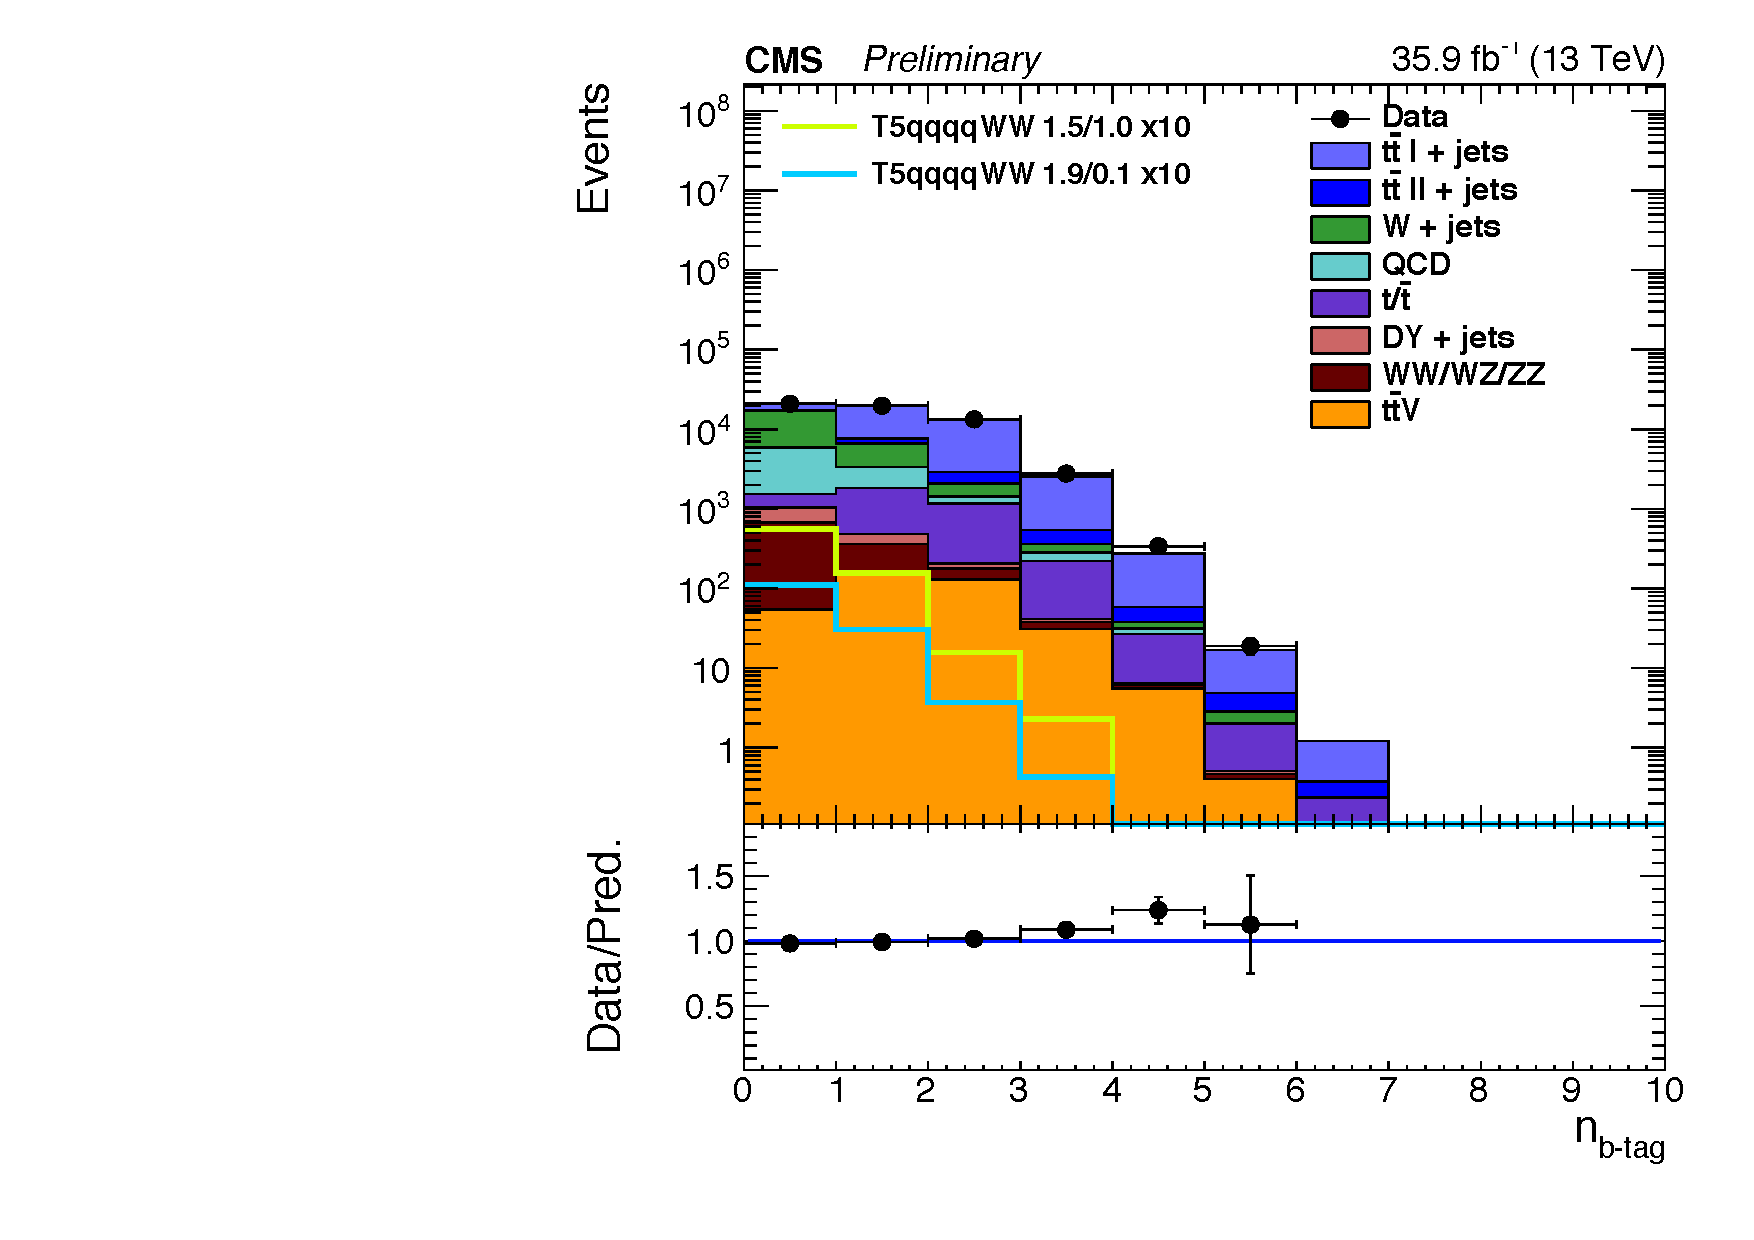
\includegraphics[width=0.45 \textwidth]{Plots/analysis/control_Plots/nBjet0b}
 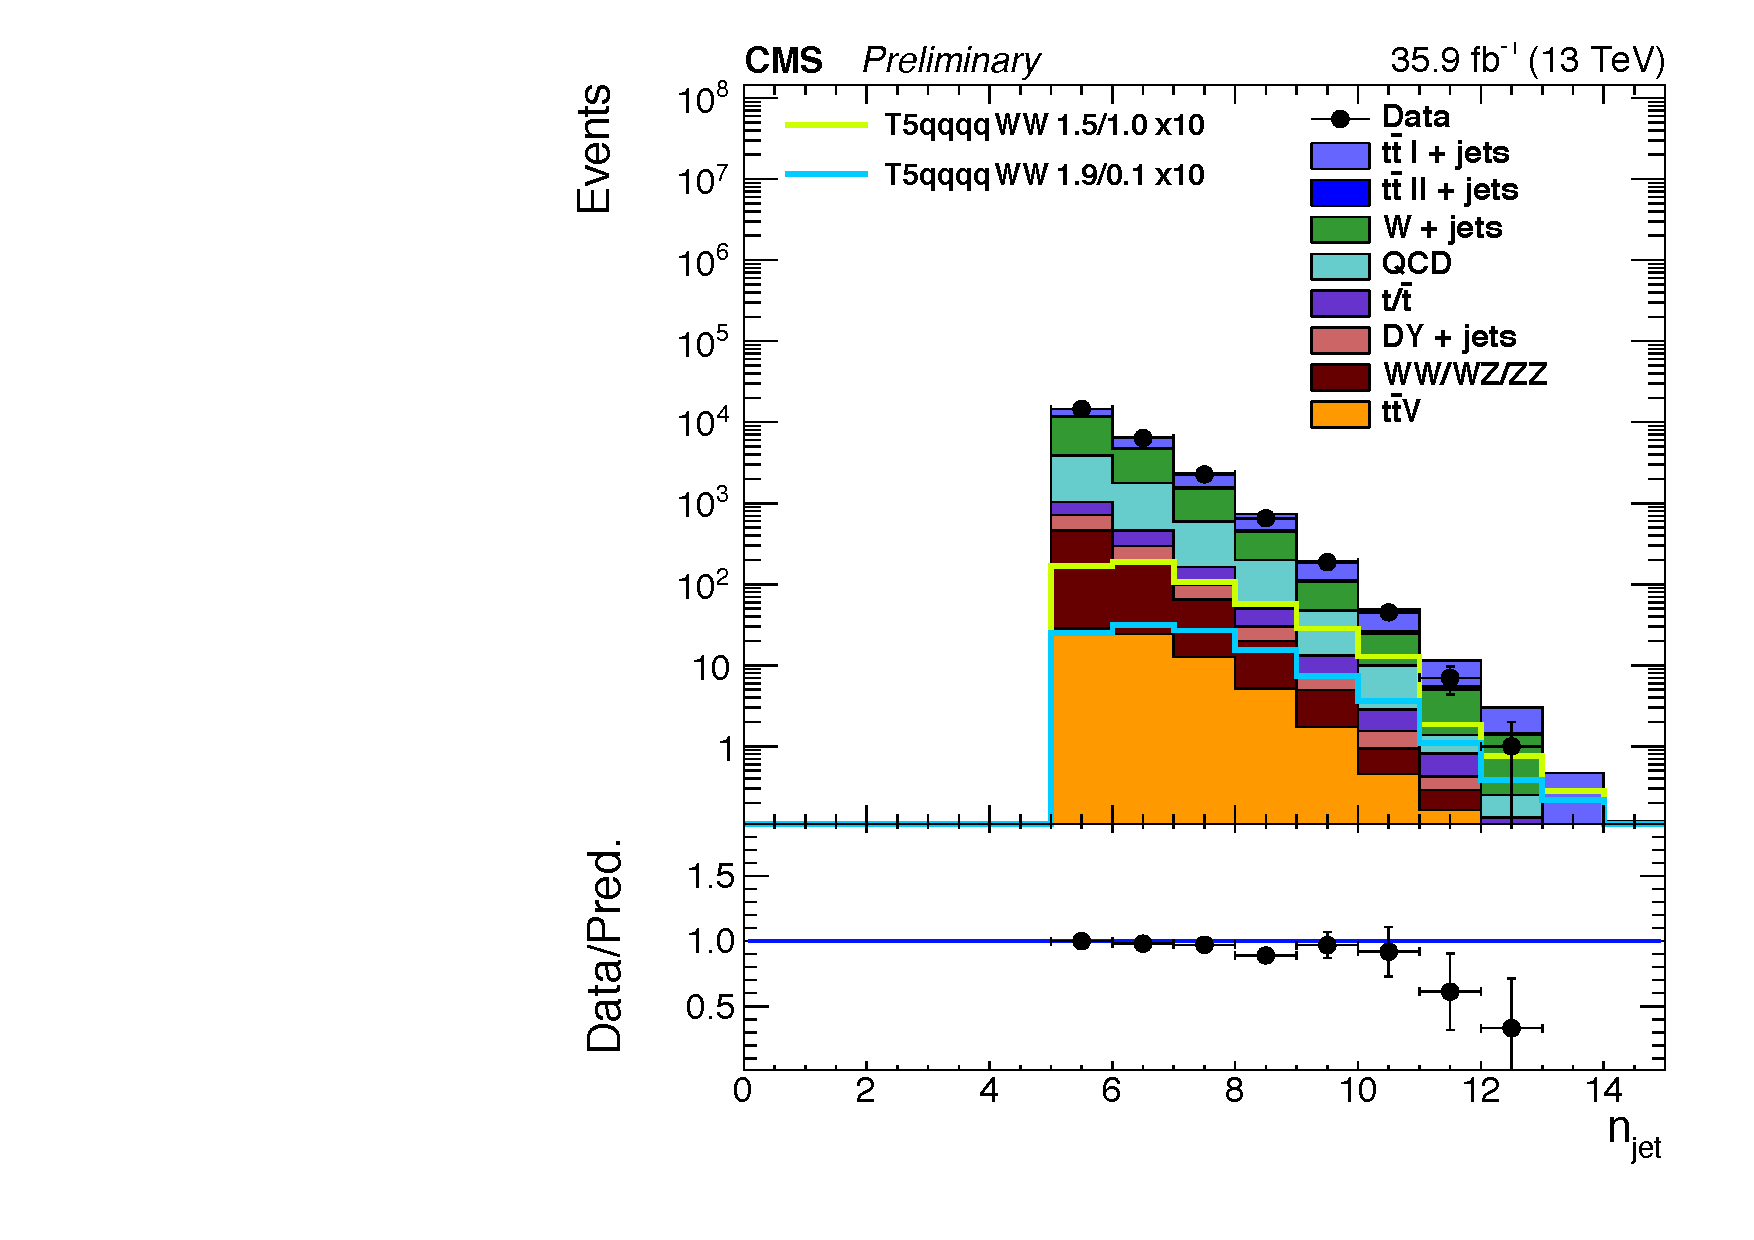
\includegraphics[width=0.45 \textwidth]{PhD_Thesis_v4/Plots/analysis/control_Plots/plots_zerob_st250_ht500_njet5_nbtagEq0_nJet30Preliminary.pdf}\\
 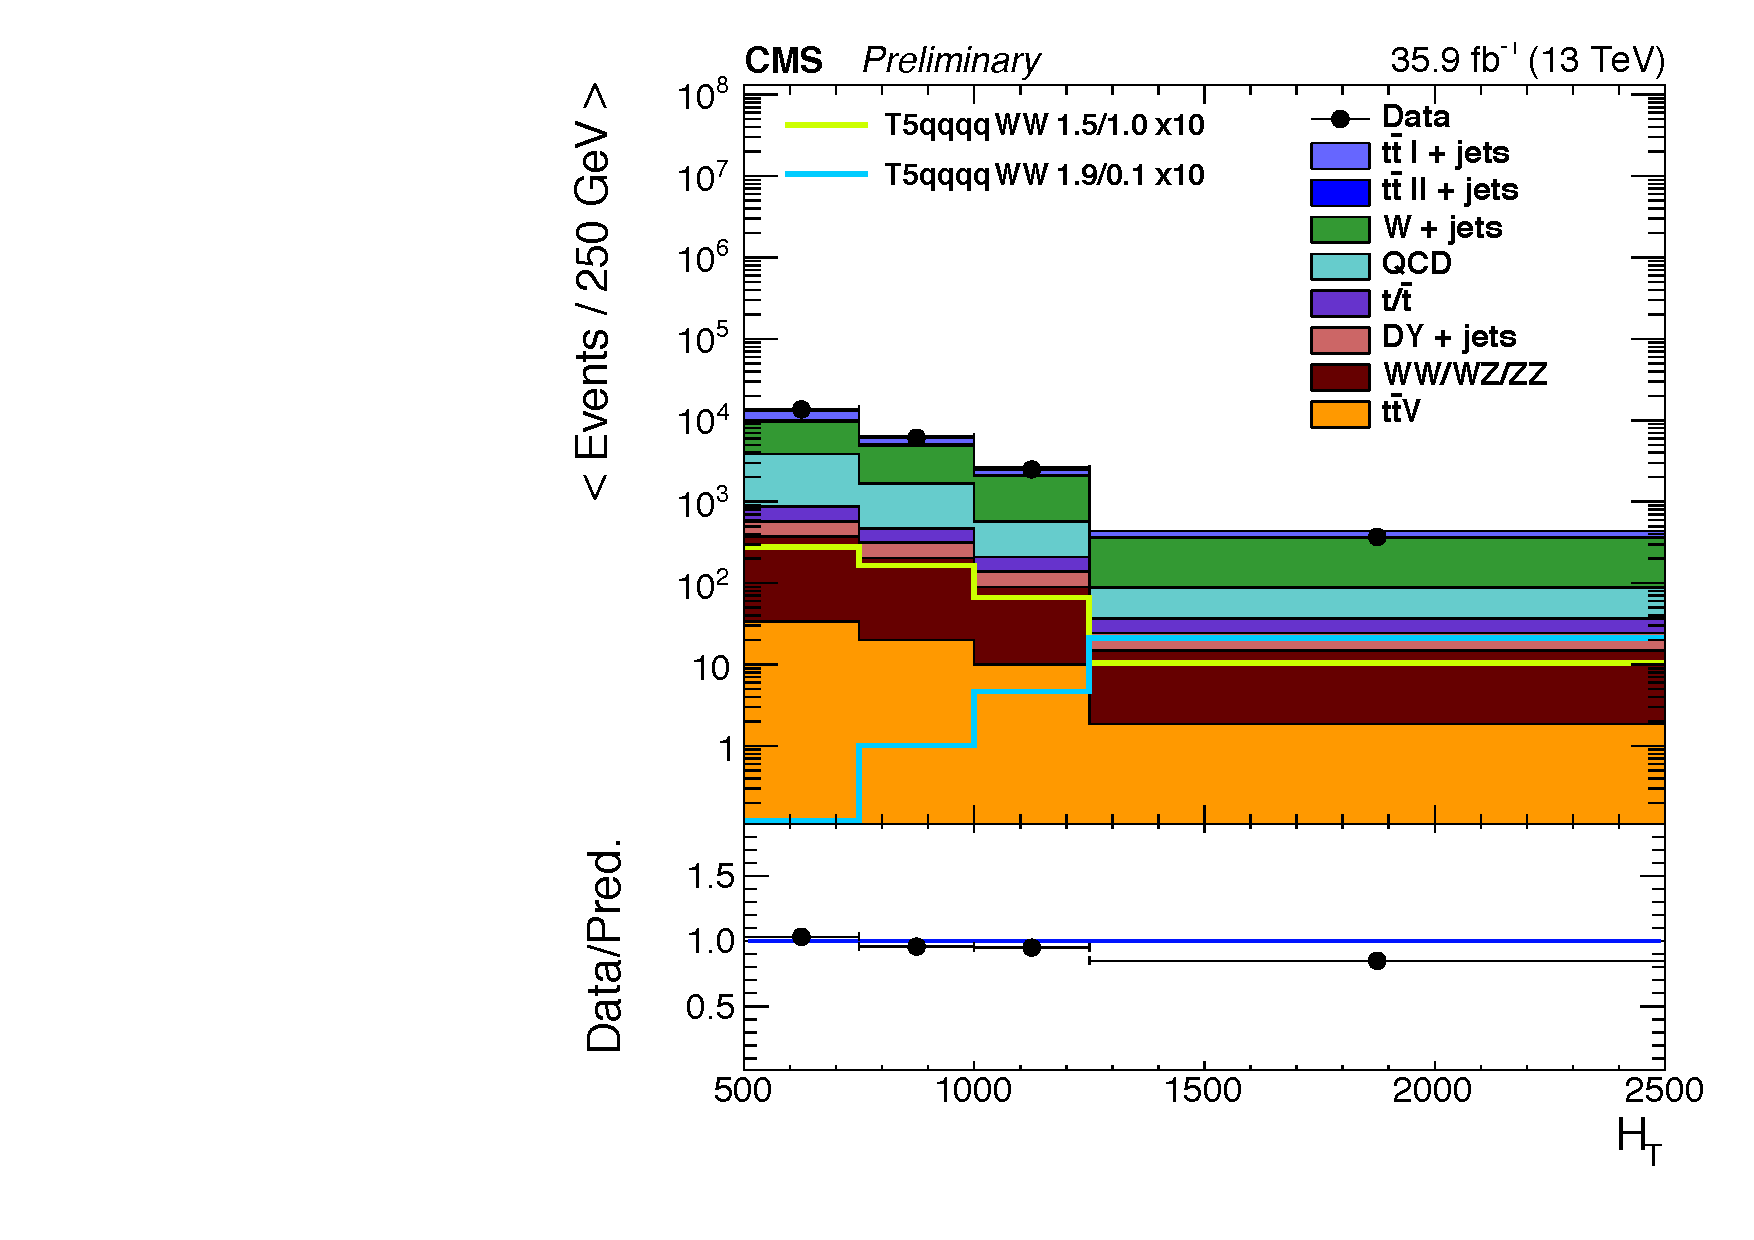
\includegraphics[width=0.45 \textwidth]{Plots/analysis/control_Plots/plots_zerob_st250_ht500_njet5_nbtagEq0_htJet30jPreliminary}
 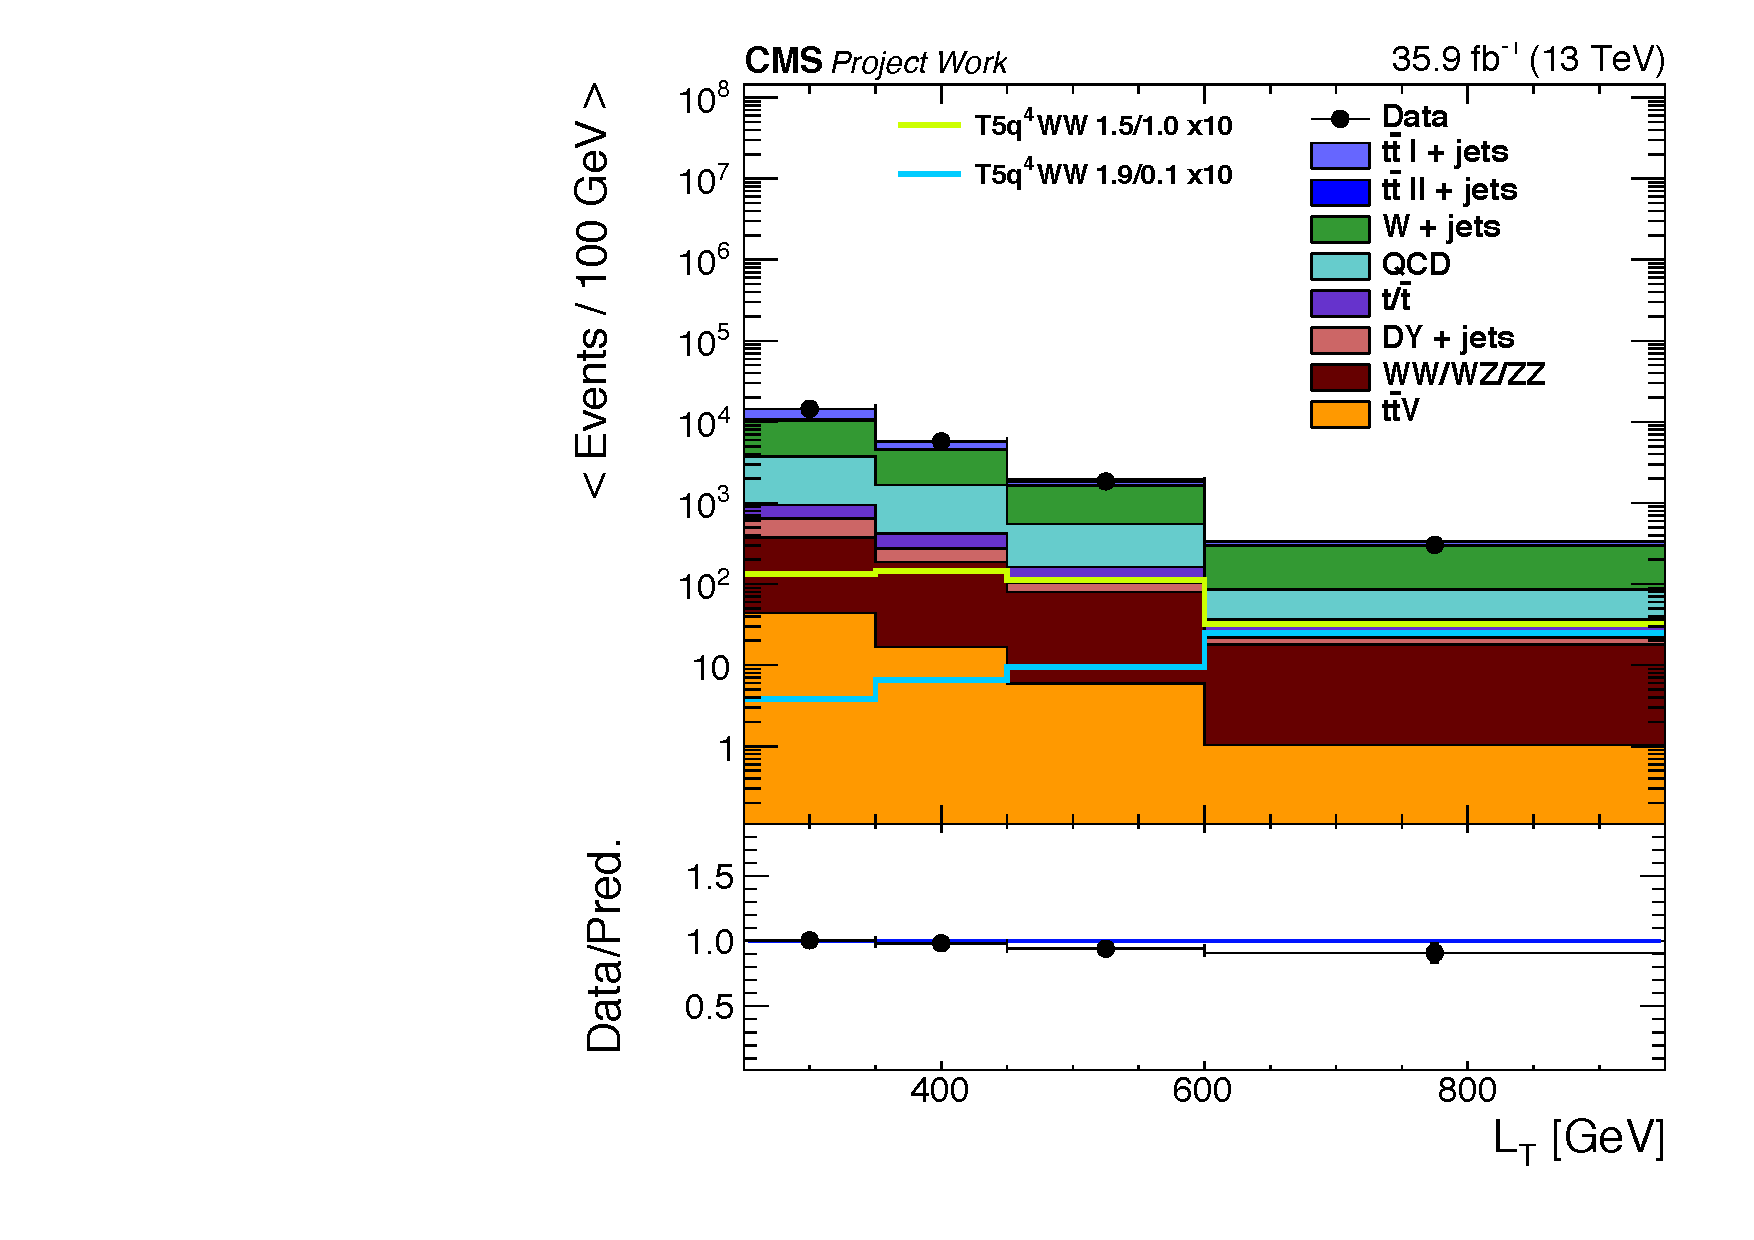
\includegraphics[width=0.45 \textwidth]{Plots/analysis/control_Plots/LT_colors}
 %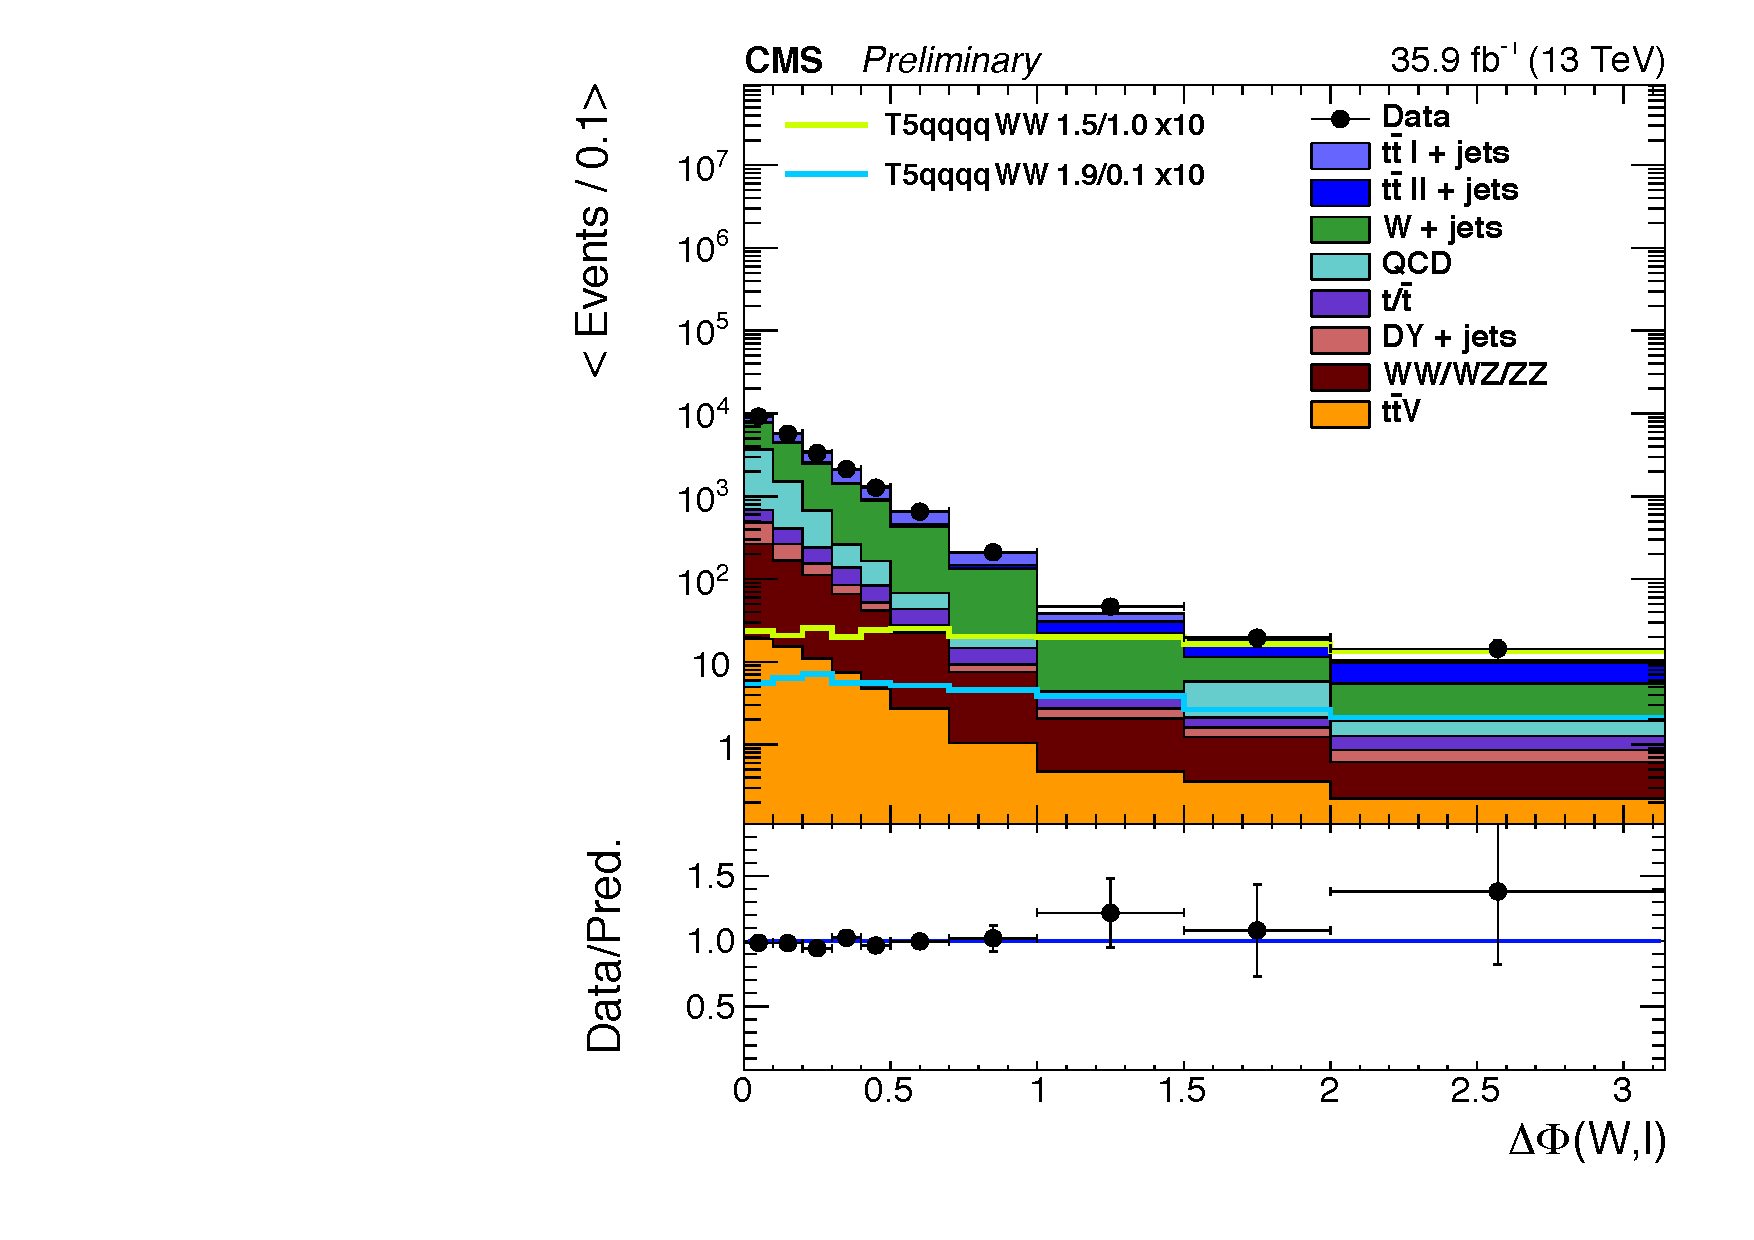
\includegraphics[width=0.45 \textwidth]{Plots/analysis/control_Plots/plots_zerob_st250_ht500_njet5_nbtagEq0_deltaPhi_WlPreliminary}
  \caption[Main kinematic distributions after baseline selection]{ \label{fig:baselineplots} Number of b-tagged jets~(top left), after the baseline selection, requiring at least five jets, minimum $\HT$ of 500~GeV, a minimum $\LT$ of 250~GeV and exactly one lepton with $\pt >$25~GeV. The other distributions~(top right and bottom) shown with an additional b jet veto. Number of jets distribution~(top right), $\HT$~(bottom left) and $\LT$~(bottom right) are shown.
  %The top left distribution shows the number of . The rest of the distributions are plotted after the same baseline selection additionally requiring no b-tagged jets. In the top row the number of jets (right) while in the bottom row $\HT$ (left) and $\LT$ (right) distributions are shown. The simulated background events are stacked on top of each other, and several signal points are overlaid for illustration without being stacked. The model T5qqqqWW (1.5,1.0) (T5qqqqWW (1.9,0.1)) corresponds to a gluino mass of 1.5 TeV (1.9 TeV) and neutralino mass of 1.1 TeV (0.1 TeV), respectively. The intermediate chargino mass is fixed at 1.25 TeV (1.0 TeV).
  The benchmark signal models are scaled up by a factor of 10.
  }
   \end{center}
\end{figure*}
\chapter{Design of Search Regions}
Explain MB , SB...  
\newpage
\section{Signal Regions}
\subsection{Background and Signal composition in MB SR}
\newpage
\section{Control Regions}
\subsection{Background composition in MB CR and SB SR/CR}
\newpage
\newpage
\subsection{Signal contamination in MB CR and SB SR/CR}
Tell that It is negligible
\newpage
